\PassOptionsToPackage{hyperfootnotes=false}{hyperref}
\documentclass[a4paper,fleqn]{cas-sc}
\usepackage[pagewise]{lineno}
% \linenumbers

\usepackage[numbers]{natbib}
\usepackage{subfiles}
\usepackage[version=4]{mhchem}
\usepackage{cleveref}
\usepackage{subcaption}
\usepackage{longtable}
\usepackage{mathtools}
\usepackage{tabularx}
\usepackage{makecell}
\usepackage{booktabs}
\usepackage{adjustbox}
\usepackage{xspace}
\renewcommand\cellalign{tl}
\newcolumntype{P}[1]{>{\centering\arraybackslash}p{#1}}
\usepackage{listings}
\usepackage{xcolor}
\usepackage{color}
\usepackage{siunitx}
\graphicspath{{figures/}}

\definecolor{dkgreen}{rgb}{0,0.6,0}
\definecolor{gray}{rgb}{0.5,0.5,0.5}
\definecolor{mauve}{rgb}{0.58,0,0.82}

\lstset{
    frame=tb,
    language=Python,
    aboveskip=3mm,
    belowskip=3mm,
    showstringspaces=false,
    columns=flexible,
    basicstyle={\small\ttfamily},
    numbers=none,
    numberstyle=\tiny\color{gray},
    keywordstyle=\color{blue},
    commentstyle=\color{dkgreen},
    stringstyle=\color{mauve},
    breaklines=true,
    breakatwhitespace=true,
    tabsize=3
}

\newcommand{\Ha}{\text{Ha}}
\newcommand{\COtwo}{\ce{CO2}\xspace}
\newcommand{\HtwoO}{\ce{H2O}\xspace}
\newcommand{\MEA}{\ce{MEA}\xspace}
\newcommand{\MEAH}{\ce{MEAH+}\xspace}
\newcommand{\MEACOO}{\ce{MEACOO-}\xspace}
\newcommand{\HCOthree}{\ce{HCO3-}\xspace}
\newcommand{\COthree}{\ce{CO3^2-}\xspace}
\newcommand{\HthreeO}{\ce{H3O+}\xspace}
\newcommand{\Hydroxide}{\ce{OH-}\xspace}
\newcommand{\Ntwo}{\ce{N2}\xspace}
\newcommand{\Otwo}{\ce{O2}\xspace}
\newcommand{\NtwoO}{\ce{N2O}\xspace}

\newcommand{\A}{\text{A}}
\newcommand{\B}{\text{B}}
\newcommand{\C}{\text{C}}
\newcommand{\D}{\text{D}}
\newcommand{\code}[1]{\texttt{#1}}
\newcommand{\liq}{\ell}
\newcommand{\vap}{v}

\begin{document}

\let\WriteBookmarks\relax
\def\floatpagepagefraction{1}
\def\textpagefraction{.001}

\shorttitle{SSM+DS ePC-SAFT Evaluation for Aqueous MEA}
\shortauthors{Polley}

\title[mode = title]{\texorpdfstring{Evaluation of SSM+DS Modified-Born ePC-SAFT for \ce{CO2} Solubility and Speciation in Aqueous Monoethanolamine}{Evaluation of SSM+DS Modified-Born ePC-SAFT for CO2 Solubility and Speciation in Aqueous Monoethanolamine}}

\author[1]{Tanner W. Polley}[orcid=0009-0008-5957-4152]
\cormark[1]
\ead{tpolley3@byu.edu}

\affiliation[1]{
    organization={Department of Chemical Engineering, Brigham Young University},
    city={Provo},
    state={UT},
    postcode={84602},
    country={United States}
}

\cortext[cor1]{Corresponding author.}

\begin{abstract}
Reactive \COtwo absorption couples equilibrium gas pressure to aqueous electrolyte composition.  We developed a solvation-shell-modeling plus dielectric-saturation (SSM+DS) modified-Born electrolyte perturbed-chain statistical associating fluid theory (ePC-SAFT) model for \COtwo solubility and speciation in 30 wt\% aqueous monoethanolamine (\MEA).  A five-reaction liquid model resolved \COtwo, \MEA, \HtwoO, \MEAH, \MEACOO, \HCOthree, \COthree, \HthreeO, and \Hydroxide.  Seven \MEAH/\MEACOO parameters were fitted to 22 composition residuals from eight nuclear magnetic resonance states; the remaining parameters were taken from literature.  Model evaluation used 161 vapor--liquid-equilibrium pressure records and 66 additional speciation states over 20--\SI{120}{\degreeCelsius} and \COtwo loadings of 0.003--0.990.  On 31 Jou et al.\ measurements common to an ideal-activity baseline and the ePC-SAFT calculation, the median absolute \(\log_{10}(P_{\mathrm{model}}/P_{\mathrm{data}})\) residual was 0.160 for the ideal baseline and 0.495 for ePC-SAFT.  The ePC-SAFT calculation converged for all experimental states.  On the 66 speciation states excluded from parameter estimation, median absolute residuals for positive measurements were 0.065 for \MEA, 0.033 for \MEAH, 0.041 for \MEACOO, and 0.452 for \HCOthree.  The model described amine-family speciation more closely than pressure or carbonate speciation.
\end{abstract}

\begin{keywords}
\COtwo solubility\sep{}ePC-SAFT\sep{}SSM+DS modified Born\sep{}monoethanolamine\sep{}reactive vapor--liquid equilibrium\sep{}electrolyte speciation
\end{keywords}

\maketitle

\hypersetup{
    pdftitle={Evaluation of SSM+DS Modified-Born ePC-SAFT for CO2 Solubility and Speciation in Aqueous Monoethanolamine},
    pdfauthor={Tanner W. Polley},
    pdfsubject={Reactive aqueous MEA-CO2-H2O thermodynamics with modified-Born ePC-SAFT},
    pdfkeywords={carbon dioxide, monoethanolamine, ePC-SAFT, modified Born, speciation, vapor-liquid equilibrium}
}

\section{Introduction}\label{sec:introduction}
\COtwo solubility in aqueous alkanolamines is a central thermodynamic quantity for carbon-capture solvents.  Monoethanolamine (\MEA) remains a reference solvent because of its industrial history and extensive experimental literature.  Absorbed \COtwo reacts with water and amine to form molecular \COtwo, protonated amine, carbamate, bicarbonate, carbonate, hydronium, and hydroxide.  The equilibrium \COtwo pressure at a given loading consequently depends on both phase equilibrium and liquid speciation.

Reactive vapor--liquid-equilibrium measurements commonly express \COtwo solubility as partial pressure versus loading.  Pressure measurements test the gas--liquid fugacity balance, while spectroscopic composition measurements test reaction equilibria, material balances, and electroneutrality.  Fitting pressure alone can conceal an implausible distribution of \MEA, \MEAH, \MEACOO, \HCOthree, and \COthree.  We therefore evaluate pressure and speciation as coupled observations of the same thermodynamic state.

\subsection{CO2 solubility in reactive MEA}
Experimental data often specify unloaded amine mass fraction and absorbed \COtwo per mole of amine.  Material and charge balances map these apparent variables to a true-species liquid composition before the equation of state evaluates fugacities and activity coefficients.  The evidence used here combines vapor--liquid-equilibrium (VLE) measurements of \COtwo partial pressure with nuclear magnetic resonance (NMR) measurements of liquid species.  VLE data define the pressure response, and NMR data constrain the underlying chemical composition.

\subsection{Thermodynamic modeling of CO2 solubility in MEA--CO2--H2O}
Thermodynamic descriptions of \COtwo-loaded amines have historically relied on apparent-species correlations or activity-coefficient models.  Kent--Eisenberg and related apparent-equilibrium approaches provide compact correlations with transferability limited to their fitted temperature, loading, and solvent-composition windows.  Electrolyte-NRTL and related excess-Gibbs-energy models represent ionic liquid nonideality for \MEA--\COtwo--\HtwoO systems\cite{Zhang2011,Morgan2017b,Mouhoubi2020,Hilliard2008}.  Their reliability depends on fitted interaction parameters and the species convention used for regression.

The \MEA literature contains pressure and speciation measurements suitable for testing a molecularly explicit description of \COtwo solubility.  VLE studies report \COtwo partial pressures across temperature, loading, and amine-composition conditions\cite{Jou1995,Hilliard2008,Mamun2005,Xu2011,Aronu2011}.  NMR studies report liquid-phase \MEA, \MEAH, \MEACOO, \HCOthree, and carbonate-containing observables at several levels of species resolution\cite{Jakobsen2005,Bottinger2008,Matin2012}.  A reactive-solubility model can thus be assessed against both gas pressure and liquid composition.

\subsection{SAFT and PC-SAFT models for CO2 solubility}
Statistical associating fluid theory (SAFT)-type equations of state provide an alternative to purely excess-Gibbs-energy descriptions because molecular size, dispersion, chain formation, and association are represented in the Helmholtz-energy model.  The perturbed-chain statistical associating fluid theory (PC-SAFT) equation of Gross and Sadowski introduced a perturbation theory for chain molecules\cite{Gross2001}, and its associating extension provides the site-based hydrogen-bonding contribution needed for water and alkanolamines\cite{Gross2002}.  PC-SAFT has been applied directly to aqueous ethanolamine systems and acid-gas solubility, including pure alkanolamine property regression and VLE prediction for aqueous amines\cite{Nasrifar2010}.  Baygi and Pahlavanzadeh applied PC-SAFT to \COtwo solubility in aqueous \MEA, using a chemical-equilibrium step to reconstruct liquid species and a neutral PC-SAFT pressure calculation as the phase-equilibrium model\cite{Baygi2015}.  Other SAFT variants have also been used for loaded \MEA, including transferable SAFT-VR models that represent chemisorption stoichiometry through effective association sites\cite{MacDowell2010}.  More recent SAFT comparisons for alkanolamines continue to show that EOS-based models can describe pure, binary, and ternary amine properties with physically interpretable parameters\cite{Pakravesh2025a}.

Most PC-SAFT treatments of loaded \MEA use an apparent chemistry representation or solve the reactive liquid composition outside the electrolyte EOS.  They then pass that composition to the phase-equilibrium calculation instead of deriving ionic activity coefficients from the same EOS.  This separation matters for \MEA because carbamate formation creates the \MEAH/\MEACOO ion pair absent from tertiary-amine MDEA chemistry.

\subsection{ePC-SAFT and advanced Born electrostatics}
Electrolyte PC-SAFT (ePC-SAFT) extends PC-SAFT to charged species by adding an electrolyte contribution to the residual Helmholtz energy.  The original aqueous-electrolyte formulation introduced Debye--Huckel electrostatic effects into the PC-SAFT framework and demonstrated correlations for aqueous salt densities and vapor pressures\cite{Cameretti2005}.  Uyan et al. applied ePC-SAFT to aqueous MDEA--\COtwo solubility with explicit ionic species and activity-coupled chemical equilibrium, treating the calculation as predictive when no binary parameters were adjusted to the ternary acid-gas data\cite{Uyan2015}.  Wangler et al. extended that amine-solubility strategy by fitting selected binary interactions to independent osmotic-coefficient data and validating the resulting model against acid-gas solubility, thereby distinguishing literature-collected pure-component parameters, independently regressed binary parameters, and final VLE validation data\cite{Wangler2018}.

Later ePC-SAFT developments addressed non-aqueous and mixed-solvent electrolytes, where ion solvation and composition-dependent permittivity become central.  The ePC-SAFT advanced formulation of Buelow, Ascani, and Held incorporated a concentration-dependent dielectric constant into both the Born contribution and Debye--Huckel term\cite{Bulow2020}; the second part extended the framework to salt solubility and ion pairing\cite{Bulow2021}.  Subsequent work used ePC-SAFT advanced to predict \COtwo solubility in aqueous and organic electrolyte solutions, including systems with carbonate chemistry\cite{Schick2023}.  More recent studies refined the modified-Born term through solvation-shell modeling and dielectric saturation (SSM+DS), which add ion-local solvation structure to the Born contribution\cite{Rueben2024,Figiel2025}.

Loaded aqueous \MEA tests this model class because \COtwo loading changes the ionic population, solvent dielectric environment, and carbamate concentration.  The system combines associating neutral molecules, molecular \COtwo, changing solvent composition, and several ionic products of acid--base chemistry.  A true-species SSM+DS ePC-SAFT model links phase equilibrium, reaction equilibrium, ionic activity coefficients, and composition-dependent solvation within one thermodynamic framework.

\begin{table*}
    \centering
    \scriptsize
    \caption{Positioning of the present \MEA \COtwo-solubility study relative to representative SAFT-family and electrolyte-model studies.}
    \label{tab:literature-model-comparison}
    \begin{tabularx}{\textwidth}{@{}>{\raggedright\arraybackslash}p{2.2cm}>{\raggedright\arraybackslash}X>{\raggedright\arraybackslash}X>{\raggedright\arraybackslash}X>{\raggedright\arraybackslash}X@{}}
        \toprule
        Study & System and model & Species and activity treatment & Data and fitted quantities & Validation reported \\
        \midrule
        Nasrifar and Tafazzol\cite{Nasrifar2010} & \MEA--\HtwoO and acid-gas PC-SAFT mixtures & Apparent neutral mixture basis without explicit Born treatment & Pure-component and VLE/property data; molecular parameters and binary interactions & Pure and mixture thermodynamic-property checks \\
        Baygi and Pahlavanzadeh\cite{Baygi2015} & \MEA--\HtwoO--\COtwo PC-SAFT with external chemistry & Six-species reconstructed liquid without ionic ePC-SAFT activity coupling or SSM+DS Born terms & \COtwo pressure data with reconstructed speciation; neutral PC-SAFT molecular and binary terms & Pressure curves and reconstructed speciation \\
        Uyan et al.\cite{Uyan2015} & MDEA--\HtwoO--\COtwo ePC-SAFT & Explicit ionic true-species chemistry with electrolyte activity terms; no \MEA carbamate ion pair & Solubility data and independent parameter sources; selected ion and binary parameters & Predictive ternary acid-gas solubility checks \\
        Wangler et al.\cite{Wangler2018} & MDEA amine ePC-SAFT systems & Explicit ionic true species with fitted electrolyte binary interactions; no \MEACOO pathway & Osmotic, solubility, and related data; selected binary and pure-ion quantities & Acid-gas solubility and related validation data \\
        Buelow et al.\cite{Bulow2020,Bulow2021} & Electrolyte and mixed-solvent advanced ePC-SAFT & Concentration-dependent permittivity with advanced Born corrections & Electrolyte solution and salt-solubility data; dielectric/Born framework terms & Electrolyte and salt-solubility validation \\
        Figiel et al.\cite{Figiel2025} & Electrolyte and organic-solvent modified-Born ePC-SAFT & Explicit ionic true species with SSM+DS modified Born treatment & Electrolyte activity and solubility data; Born, dielectric, and solvent-shell conventions & Activity, solubility, and consistency checks \\
        This work & \MEA--\HtwoO--\COtwo SSM+DS modified-Born ePC-SAFT & Nine-species explicit ionic basis with \MEAH/\MEACOO carbamate chemistry, SSM+DS Born terms, and concentration-dependent permittivity & 161 \COtwo-solubility pressure rows and 74 NMR-derived speciation rows; direct \MEAH/\MEACOO ion regression and fixed-parameter activity evaluation & Solubility-pressure/speciation residuals, train-validation split, and carbonate Born identifiability screen \\
        \bottomrule
    \end{tabularx}
\end{table*}


\subsection{Contribution of this work}
We develop a nine-species SSM+DS modified-Born ePC-SAFT model for reactive aqueous \MEA--\HtwoO--\COtwo.  The calculation couples reaction equilibria to ePC-SAFT activities, fugacities, concentration-dependent permittivity, and modified-Born solvation.  We fit the \MEAH/\MEACOO parameters to NMR speciation measurements, then evaluate the resulting model against additional NMR states and 161 \COtwo partial-pressure records.  The comparison tests both the equilibrium pressure and the liquid species distribution predicted by one thermodynamic state.

\section{Theory}\label{sec:theory}
We formulate \COtwo solubility as a reacting electrolyte vapor--liquid-equilibrium problem.  At specified temperature, apparent amine concentration, and absorbed \COtwo loading, the calculation determines a charge-balanced true-species liquid composition and the corresponding vapor-phase \COtwo partial pressure.  The liquid composition enters the ePC-SAFT fugacity coefficients, activity coefficients, and electrostatic contributions.

\subsection{PC-SAFT residual Helmholtz energy}
ePC-SAFT is formulated as a residual Helmholtz-energy equation of state.  For a state defined by temperature \(T\), molar density \(\rho\), and mole-fraction vector \(\boldsymbol{x}\), the reduced residual Helmholtz energy \(\tilde{a}^{\mathrm{res}}=a^{\mathrm{res}}/(RT)\) is assembled from hard-chain, dispersion, association, Debye--Huckel, and Born terms \cite{Gross2001,Gross2002,Cameretti2005,Bulow2021a,Figiel2025}:
\begin{equation}
    \tilde{a}^{\mathrm{res}}
    =
    \tilde{a}^{\mathrm{hc}}
    +\tilde{a}^{\mathrm{disp}}
    +\tilde{a}^{\mathrm{assoc}}
    +\tilde{a}^{\mathrm{DH}}
    +\tilde{a}^{\mathrm{Born}} ,
    \label{eq:epcsaft-residual-split}
\end{equation}
The hard-chain contribution represents the repulsive chain reference, dispersion represents short-range attraction, association represents site-specific hydrogen bonding, the Debye--Huckel term represents long-range electrostatics, and the Born term represents electrostatic solvation.  In loaded \MEA, neutral solvent structure, ionic strength, and solvation all change with \COtwo loading.  Neutral \MEA and \HtwoO require segment, dispersion, and association parameters; charged species also require charge, dielectric, and Born-diameter information.

The hard-chain reference is built from packing-fraction moments
\begin{equation}
    \zeta_n=\frac{\pi}{6}\rho\sum_i x_i m_i d_i^n,\qquad n\in\{0,1,2,3\},
    \label{eq:epcsaft-zeta-moments}
\end{equation}
where \(m_i\) is the segment number and \(d_i\) is the temperature-dependent segment diameter.  With \(\bar{m}=\sum_i x_i m_i\), the chain correction subtracts the connectivity penalty from the hard-sphere reference,
\begin{equation}
    \tilde{a}^{\mathrm{hc}}
    =
    \bar{m}\tilde{a}^{\mathrm{hs}}
    -
    \sum_i x_i(m_i-1)\ln g_{ii}^{\mathrm{hs}}(\sigma_{ii}) .
    \label{eq:epcsaft-hard-chain}
\end{equation}
The hard-chain term sets the excluded-volume and density scales that enter fugacity and liquid-state activity coefficients.

The dispersion term introduces attractive perturbations through mixture moments of segment energy and size,
\begin{equation}
    \tilde{a}^{\mathrm{disp}}
    =
    -2\pi\rho I_1(\eta,\bar{m})\overline{m^2\epsilon\sigma^3}
    -\pi\rho\bar{m}C_1 I_2(\eta,\bar{m})
    \overline{m^2\epsilon^2\sigma^3},
    \label{eq:epcsaft-dispersion}
\end{equation}
Here \(\eta=\zeta_3\), \(I_1\) and \(I_2\) are the PC-SAFT dispersion integrals, and the overbars denote pair-mixed composition averages.  Binary interaction parameters modify the mixed dispersion energy \(\epsilon_{ij}\), which links pressure residuals to neutral--neutral and ion--molecule dispersion choices.

Association is represented through site fractions \(X^{A_i}\),
\begin{equation}
    \tilde{a}^{\mathrm{assoc}}
    =
    \sum_i x_i \sum_{A_i}
    \left[
        \ln X^{A_i}
        -\frac{X^{A_i}}{2}
        +\frac{1}{2}
    \right],
    \label{eq:epcsaft-association}
\end{equation}
with association strengths proportional to
\begin{equation}
    \Delta^{A_iB_j}_{ij}
    =
    d_{ij}^{3}g_{ij}^{\mathrm{hs}}
    \kappa^{A_iB_j}_{ij}
    \left[
        \exp\left(\frac{\epsilon^{A_iB_j}_{ij}}{k_{\mathrm{B}}T}\right)-1
    \right].
    \label{eq:epcsaft-association-strength}
\end{equation}
This contribution represents hydrogen bonding in water and alkanolamines.  Ions without assigned association sites contribute no association-site balances.

\subsection{Electrolyte PC-SAFT and ion activity coefficients}
For charged species, the Debye--Huckel contribution uses the dielectric state and the inverse Debye length,
\begin{align}
    \kappa
    &=
    \left[
        \frac{\rho e^2}{k_{\mathrm{B}}T\varepsilon_0\varepsilon_r}
        \sum_j x_j z_j^2
    \right]^{1/2},
    \label{eq:epcsaft-debye-kappa} \\
    \tilde{a}^{\mathrm{DH}}
    &=
    -\frac{\kappa e^2}{12\pi\varepsilon_0\varepsilon_r k_{\mathrm{B}}T}
    \sum_i x_i z_i^2\chi_i ,
    \label{eq:epcsaft-debye-helmholtz}
\end{align}
Here \(z_i\) is the ionic charge and \(\chi_i\) is the finite-ion-size correction.  Relative permittivity \(\varepsilon_r\) enters both the Debye--Huckel and Born terms.  Their residual chemical potentials determine the ePC-SAFT activity coefficients used in the liquid reaction equations.

\subsection{Modified Born term with solvation shell and dielectric saturation}
The Born contribution is evaluated in modular form:
\begin{equation}
    \tilde{a}^{\mathrm{Born}}
    =
    -\frac{e^2}{4\pi\varepsilon_0 k_{\mathrm{B}}T}
    \sum_i x_i z_i^2
    \sum_{\delta\in\mathcal{D}}
    \left(1-\frac{1}{\varepsilon_{r,m_\delta}}\right)
    D_{i,\delta}^{(m_\delta)} .
    \label{eq:epcsaft-born-modular}
\end{equation}
The active set \(\mathcal{D}\) contains the base Born term and may include solvation-shell-modeling (SSM) and dielectric-saturation (DS) corrections,
\begin{equation}
    \mathcal{D}
    =
    \{\mathrm{Born}\}\cup\mathcal{D}_{\mathrm{add}},
    \qquad
    \mathcal{D}_{\mathrm{add}}\subseteq\{\mathrm{SSM},\mathrm{DS}\}.
    \label{eq:epcsaft-born-active-set}
\end{equation}
For SSM+DS, \(\mathcal{D}_{\mathrm{add}}=\{\mathrm{SSM},\mathrm{DS}\}\).  The base Born and SSM terms use the bulk dielectric medium, while the DS term uses the ion-local dielectric medium:
\begin{equation}
    m_\delta=
    \begin{cases}
        \mathrm{bulk}, & \delta\in\{\mathrm{Born},\mathrm{SSM}\},\\
        \mathrm{ion}, & \delta=\mathrm{DS}.
    \end{cases}
    \label{eq:epcsaft-born-medium}
\end{equation}
The inverse-diameter terms are
\begin{align}
    D_{i,\mathrm{Born}}^{(\mathrm{bulk})}
    &=
    \frac{1}{d_i^{\mathrm{Born}}},
    \label{eq:epcsaft-born-base-dterm}\\
    D_{i,\mathrm{SSM}}^{(\mathrm{bulk})}
    &=
    \frac{1}{d_i^{\mathrm{Born}}+\Delta d_i}
    -
    \frac{1}{d_i^{\mathrm{Born}}},
    \label{eq:epcsaft-born-ssm-dterm}\\
    D_{i,\mathrm{DS}}^{(\mathrm{ion})}
    &=
    \frac{1}{d_i^{\mathrm{Born}}}
    -
    \frac{1}{d_i^{\mathrm{Born}}+\Delta d_i},
    \label{eq:epcsaft-born-ds-dterm}
\end{align}
with shell shift
\begin{equation}
    \Delta d_i
    =
    \frac{f_{\mathrm{mix}}-1}{|z_i|}\,d_i^{\mathrm{Born}},
    \qquad
    f_{\mathrm{mix}}=\sum_k x_k f_k .
    \label{eq:epcsaft-born-shell-shift}
\end{equation}
The SSM term changes the effective Born radius in the bulk medium, and the DS term assigns the complementary radius increment to the ion-local dielectric medium.  Carbonation changes both the ionic population and solvent environment, so both contributions vary with loading.

We use concentration-dependent bulk permittivity and the SSM+DS convention of Figiel et al.\ \cite{Figiel2025}.  That convention assigns pure ions \(\varepsilon_r=8\) and \(f_k=1\), while solvent \(f_k\) values are fitted to electrolyte activity data; reported values are 1.5 for water, 1.4 for methanol, and 1.6 for ethanol.  Hajj et al.\ measured loaded 30 wt\% \MEA over 915--2450 MHz and obtained a zero-frequency parameter by fitting a Cole--Cole dispersion model\cite{Hajj2024}.  The microwave extrapolation does not independently identify the \MEA solvent-shell parameter, so the present calculation keeps \(f_{\MEA}=1\).  With concentration-dependent permittivity, ion solvation responds to the changes in solvent composition and ionic strength produced by carbonation.  \Cref{tab:full-ionic-ssm-ds-parameters} lists the adopted \MEA-family inputs and electrolyte-literature conventions.

\subsection{MEA--CO2--H2O reaction network}
The unloaded \MEA mass fraction \(w_{\MEA}\) and \COtwo loading \(\alpha\), defined as moles of absorbed \COtwo per mole of total amine, specify the apparent feed.  Molecular-weight conversion gives the unloaded liquid composition:
\begin{equation}
    x_{\MEA,0}
    =
    \frac{w_{\MEA}}
    {M_{\MEA}/M_{\HtwoO}+w_{\MEA}\left(1-M_{\MEA}/M_{\HtwoO}\right)},
    \qquad
    x_{\HtwoO,0}=1-x_{\MEA,0}.
    \label{eq:unloaded-mea-composition}
\end{equation}
We add absorbed \COtwo according to \(n_{\COtwo,0}=\alpha n_{\MEA,0}\) and normalize the apparent state before solving the reactions.

The true-species liquid basis resolves the apparent \MEA and \COtwo inventories into the molecular and ionic species used for acid--base and solubility calculations:
\begin{equation}
    \boldsymbol{x}
    =
    \left(
    x_{\COtwo},x_{\MEA},x_{\HtwoO},x_{\MEAH},x_{\MEACOO},
    x_{\HCOthree},x_{\COthree},x_{\HthreeO},x_{\Hydroxide}
    \right).
    \label{eq:true-species-vector}
\end{equation}
The speciation calculation uses the five independent liquid reactions in \cref{tab:reaction-equilibrium-constants}.  For reaction \(r\), thermodynamic equilibrium is written in terms of activities,
\begin{equation}
    \sum_i \nu_{ri}\ln a_i = \ln K_r(T),
    \qquad
    a_i = \gamma_i^{\mathrm{ePC-SAFT}} x_i,
    \label{eq:activity-reaction-equilibrium}
\end{equation}
where $\nu_{ri}$ is the stoichiometric coefficient and $\gamma_i^{\mathrm{ePC-SAFT}}$ is the activity coefficient evaluated from the ePC-SAFT liquid state.  The reaction constants are represented as
\begin{equation}
    \ln K_r(T)=A_r+\frac{B_r}{T}+C_r\ln T+D_rT,
    \label{eq:reaction-equilibrium-constant-temperature}
\end{equation}
with \(T\) in kelvin and a mole-fraction activity convention.  \Cref{tab:reaction-equilibrium-constants} gives the source range of each coefficient correlation.  The ideal baseline replaces each activity coefficient with unity.

\begin{table*}[t]
    \centering
    \scriptsize\rmfamily
    \setlength{\tabcolsep}{3pt}
    \renewcommand{\arraystretch}{1.12}
    \caption{Liquid-phase reaction network and equilibrium-constant coefficients used for the activity-coupled speciation solve.  The constants use \(\ln K_r(T)=A_r+B_r/T+C_r\ln T+D_rT\), with \(T\) in kelvin and \(a_i=\gamma_i x_i\) on a mole-fraction activity basis.  Coefficients are taken from the acid-gas/ethanolamine reaction basis used in PC-SAFT calculations~\cite{Nasrifar2010}.}
    \label{tab:reaction-equilibrium-constants}
    \begin{adjustbox}{max width=\textwidth}
    \begin{tabularx}{\textwidth}{@{}c>{\raggedright\arraybackslash}Xcccccc@{}}
        \toprule
        ID & Liquid reaction & Source constant & \(A_r\) & \(B_r\) & \(C_r\) & \(D_r\) & Source range (K) \\
        \midrule
        R1 & \(2\HtwoO \rightleftharpoons \HthreeO+\Hydroxide\) & \(k_1^x\) & 132.899 & -13445.9 & -22.4773 & 0 & 273--498 \\
        R2 & \(\COtwo+2\HtwoO \rightleftharpoons \HCOthree+\HthreeO\) & \(k_2^x\) & 231.456 & -12092.1 & -36.7816 & 0 & 273--498 \\
        R3 & \(\HCOthree+\HtwoO \rightleftharpoons \COthree+\HthreeO\) & \(k_3^x\) & 216.049 & -12431.7 & -35.4819 & 0 & 273--498 \\
        R4 & \(\MEACOO+\HtwoO \rightleftharpoons \MEA+\HCOthree\) & \(k_9^x\) & 2.8898 & -3635.09 & 0 & 0 & 298--393 \\
        R5 & \(\MEAH+\HtwoO \rightleftharpoons \MEA+\HthreeO\) & \(k_7^x\) & 2.1211 & -8189.38 & 0 & -0.007484 & 273--323 \\
        \bottomrule
    \end{tabularx}
    \end{adjustbox}
\end{table*}


The liquid composition also satisfies carbon, amine, and water pseudo-component balances plus electroneutrality:
\begin{align}
    x_{\COtwo,0} &= x_{\COtwo}+x_{\MEACOO}+x_{\HCOthree}+x_{\COthree}, \\
    x_{\MEA,0} &= x_{\MEA}+x_{\MEAH}+x_{\MEACOO}, \\
    x_{\HtwoO,0} &= x_{\HtwoO}+x_{\HCOthree}+x_{\COthree}+x_{\HthreeO}+x_{\Hydroxide}, \\
    x_{\MEAH}+x_{\HthreeO} &= x_{\MEACOO}+x_{\HCOthree}+2x_{\COthree}+x_{\Hydroxide}.
    \label{eq:true-species-balances}
\end{align}

\subsection{Phase-equilibrium conditions and reference states}
For a liquid state at temperature \(T\), pressure \(P\), and mole-fraction vector \(\boldsymbol{x}\), ePC-SAFT provides residual chemical potentials and fugacity coefficients.  Molecular vapor--liquid equilibrium requires equal fugacities,
\begin{equation}
    f_i^{\liq}(T,P,\boldsymbol{x}^{\liq})
    =
    f_i^{\vap}(T,P,\boldsymbol{y}^{\vap}),
    \qquad i \in \{\COtwo,\HtwoO,\MEA\},
    \label{eq:fugacity-equality}
\end{equation}
while ions remain in the liquid phase.  Residual chemical potentials connect phase equilibrium to the activity coefficients in the reaction equations:
\begin{equation}
    \ln\varphi_k
    =
    \tilde{\mu}_k^{\mathrm{res}}-\ln Z,
    \qquad
    \ln\gamma_i^{*}
    =
    \ln\varphi_i-\ln\varphi_i^{\infty},
    \label{eq:epcsaft-phi-gamma-link}
\end{equation}
where \(\varphi_i^{\infty}\) is the infinite-dilution reference fugacity coefficient for the liquid activity coefficient.  This convention places neutral and ionic activities on the same true-species reaction basis.  Each residual Helmholtz contribution therefore affects both phase equilibrium and reaction equilibrium.


\section{Data and Methods}\label{sec:data-methods}

\subsection{Experimental Solubility and Speciation Data}
The \COtwo-solubility data set contains 161 equilibrium partial-pressure records compiled from six VLE sources\cite{Aronu2011,Hilliard2008,Idris2014,Jou1995,Mamun2005,Xu2011}.  Each canonical record retains a stable source key, source filename, and one-based source-row identity in addition to amine mass fraction, temperature, \COtwo loading, and measured \COtwo pressure.  The aggregate is generated from a row-level inclusion manifest; six Xu records carry explicit nominal-temperature normalization from 100.5--\SI{101.1}{\degreeCelsius} to \SI{100}{\degreeCelsius} or 120.4--\SI{121.8}{\degreeCelsius} to \SI{120}{\degreeCelsius}.  The speciation data set contains 74 NMR-derived liquid-composition records compiled from three spectroscopic studies\cite{Bottinger2008,Jakobsen2005,Matin2012}.  The speciation records are expressed on a common loading basis and reconciled to satisfy carbon, amine, water, and charge balances before model comparison.

\begin{center}
    \begin{minipage}{\linewidth}
    \centering
    \captionsetup{hypcap=false}
    \captionof{table}{Experimental evidence base used for the \MEA \COtwo-solubility and speciation evaluation.}
    \label{tab:mea-data-inventory}
    \small
    \begin{tabularx}{\linewidth}{lclXX}
        \toprule
        Data family & Records & Primary sources & Conditions & Observables and residual role \\
        \midrule
        VLE & 161 & \cite{Aronu2011,Hilliard2008,Idris2014,Jou1995,Mamun2005,Xu2011} &
        30 wt\% \MEA, 40--\SI{120}{\degreeCelsius}, \(\alpha=0.003\)--0.689, \(P_{\COtwo}=1.5\times10^{-3}\)--\(2.804\times10^3\) kPa &
        Measured \COtwo pressure at fixed loading; logarithmic solubility residual \\
        Speciation & 74 & \cite{Bottinger2008,Jakobsen2005,Matin2012} &
        30 wt\% \MEA, 20--\SI{80}{\degreeCelsius}, \(\alpha=0.064\)--0.990 &
        True-species mole fractions; direct-positive, reported-zero, and balance-inferred target roles \\
        \bottomrule
    \end{tabularx}
    \end{minipage}
\end{center}

\subsection{Species Basis and Parameter Hierarchy}
The activity-based calculation uses the nine-species liquid basis defined in \cref{eq:true-species-vector}.  The parameter hierarchy separates inherited molecular parameters, SSM+DS ion conventions from modified-Born ePC-SAFT literature, provisional fixed inputs for \MEAH and \MEACOO, and trace-ion quantities retained from literature-backed or diagnostic calculations.  This hierarchy is used to evaluate a fixed advanced-Born parameter set for \COtwo-solubility modeling; it is not a pressure-only fitted model.

\begin{table}[t]
    \centering
    \caption{Full ionic ePC-SAFT component parameters used for the promoted SSM+DS MEA evaluation.}
    \label{tab:full-ionic-ssm-ds-parameters}
    \scriptsize
    \setlength{\tabcolsep}{3pt}
    \begin{tabularx}{\linewidth}{lrrrrrrr>{\raggedright\arraybackslash}X}
        \toprule
        Species & $m$ & $\sigma$ & $\epsilon/k$ & $z$ & $\varepsilon_r$ & $d^{\mathrm{Born}}$ & $f_k$ & Basis \\
        \midrule
        CO2 & 2.079 & 2.7852 & 169.21 & 0 & 1.4122 & 0 & 1 & Inherited neutral molecular parameter. \\
        MEA & 3.0353 & 3.0435 & 277.17 & 0 & 32 & 0 & 1 & Inherited associating amine; no adjusted MEA-specific $f_k$. \\
        H2O & 1.2047 & \makecell[l]{$2.7927 + 10.11\,e^{-0.01775T}$\\$- 1.417\,e^{-0.01146T}$} & 353.95 & 0 & 78.09 & 0 & 1.5 & Literature water solvent; $f_k=1.5$. \\
        MEAH+ & 1 & 3.4851 & 232.69 & 1 & 8 & 3.5332 & 1 & Fitted to Tier A MEA speciation. \\
        MEACOO- & 1 & 3.5354 & 453.27 & -1 & 8 & 3.5411 & 1 & Fitted to Tier A MEA speciation; corrected MW. \\
        HCO3- & 1 & 2.9296 & 70 & -1 & 8 & 3 & 1 & Held/Uyan bicarbonate values; regularized trace fit retained 3.0. \\
        CO3\textasciicircum{}2- & 1 & 2.4422 & 249.26 & -2 & 8 & 3 & 1 & Held/Uyan carbonate values; regularized trace fit retained 3.0. \\
        H3O+ & 1 & 3.4654 & 500 & 1 & 8 & 1.218 & 1 & Held/Uyan proton carrier with Figiel SSM+DS Born radius. \\
        OH- & 1 & 2.0177 & 650 & -1 & 8 & 3.0811 & 1 & Held/Uyan hydroxide values; hydration-derived Born diameter. \\
        \bottomrule
    \end{tabularx}
\end{table}


The parameter-evidence matrix in \cref{tab:parameter-evidence-matrix,tab:trace-parameter-evidence} distinguishes the evidentiary status of the retained inputs from trace-species quantities that are not independently identified by the available NMR targets.  The available speciation data test \MEAH and \MEACOO most directly; bicarbonate, carbonate, hydronium, and hydroxide quantities require additional caution because they are constrained by fewer direct targets or by balance relationships.

\begin{table*}[t]
    \centering
    \scriptsize
    \setlength{\tabcolsep}{3pt}
    \renewcommand{\arraystretch}{1.08}
    \caption{Parameter-evidence matrix for the primary true-species \MEA ePC-SAFT basis.}
    \label{tab:parameter-evidence-matrix}
    \begin{tabularx}{\textwidth}{>{\raggedright\arraybackslash}p{1.5cm}>{\raggedright\arraybackslash}p{3.1cm}>{\raggedright\arraybackslash}p{3.2cm}X}
        \toprule
        Species & Parameter scope & Evidence status & Data or basis \\
        \midrule
        \COtwo & \makecell[l]{$m$, $\sigma$, $\epsilon/k$,\\$\varepsilon_r$, MW} & Molecular PC-SAFT value & Non-electrolyte \COtwo parameterization used as the inherited molecular component. \\
        \MEA & \makecell[l]{$m$, $\sigma$, $\epsilon/k$,\\association terms, MW} & Molecular PC-SAFT value & Associating neutral amine parameterization retained as the \MEA molecular basis. \\
        \MEA & $f_k$ & Not adjusted in this work & Figiel et al. report solvent $f_k$ values near 1.5 for water and alcohol solvents, but the adopted \MEA calculation keeps $f_k=1$ until direct \MEA dielectric and activity evidence supports changing it. \\
        \HtwoO & \makecell[l]{$m$, $\sigma(T)$, $\epsilon/k$,\\association terms,\\$\varepsilon_r$, $f_k$, MW} & SSM+DS solvent parameter & Water PC-SAFT parameters and SSM+DS $f_k=1.5$ from modified-Born ePC-SAFT literature. \\
        \MEAH & \makecell[l]{$\sigma$, $\epsilon/k$,\\$d^{\mathrm{Born}}$} & Fitted to \MEA speciation data & Direct \MEAH NMR/speciation targets in the selected amine-ion data subset. \\
        \MEAH & \makecell[l]{$\varepsilon_r$, $f_k$,\\$z$, MW} & Ionic conventions & All ions use relative dielectric constant 8 and $f_k=1$ in SSM+DS; charge and molecular weight come from the species definition. \\
        \MEACOO & \makecell[l]{$\sigma$, $\epsilon/k$,\\$d^{\mathrm{Born}}$,\\$k_{ij}(\MEAH,\MEACOO)$} & Fitted to \MEA speciation data & Direct carbamate NMR/speciation targets in the selected amine-ion data subset; the \MEAH/\MEACOO interaction was fitted with the same subset. \\
        \MEACOO & \makecell[l]{$\varepsilon_r$, $f_k$,\\$z$, MW} & Ionic conventions plus corrected molecular weight & All ions use relative dielectric constant 8 and $f_k=1$ in SSM+DS; MW is corrected to \MEA+\COtwo-H = 0.10408 kg/mol. \\
        \bottomrule
    \end{tabularx}
\end{table*}

\begin{table*}[t]
    \centering
    \scriptsize
    \setlength{\tabcolsep}{3pt}
    \renewcommand{\arraystretch}{1.08}
    \caption{Trace-species parameter evidence retained for the true-species \MEA ePC-SAFT basis.}
    \label{tab:trace-parameter-evidence}
    \begin{tabularx}{\textwidth}{>{\raggedright\arraybackslash}p{1.5cm}>{\raggedright\arraybackslash}p{3.1cm}>{\raggedright\arraybackslash}p{3.2cm}X}
        \toprule
        Species & Parameter scope & Evidence status & Data or basis \\
        \midrule
        \HCOthree & \makecell[l]{$\sigma$, $\epsilon/k$,\\$d^{\mathrm{Born}}$,\\$\varepsilon_r$, $f_k$,\\$z$, MW} & Literature-backed trace-species set plus Born sensitivity & \HCOthree uses Held/Uyan $\sigma=2.9296$, $\epsilon/k=70.00$, and water-ion $k_{ij}=0.0$; the regularized calculation retains $d^{\mathrm{Born}}=3.0$, while an unanchored sensitivity check gives a lower-residual bicarbonate-sensitive value near 6.80. \\
        \COthree & \makecell[l]{$\sigma$, $\epsilon/k$,\\$d^{\mathrm{Born}}$,\\$\varepsilon_r$, $f_k$,\\$z$, MW} & Literature-backed trace-species set plus Born sensitivity & \COthree uses Held/Uyan $\sigma=2.4422$, $\epsilon/k=249.26$, and water-ion $k_{ij}=-0.25$; the regularized calculation retains $d^{\mathrm{Born}}=3.0$. \\
        \HthreeO & \makecell[l]{$\sigma$, $\epsilon/k$,\\$d^{\mathrm{Born}}$,\\$\varepsilon_r$, $f_k$,\\$z$, MW} & Literature-backed proton-carrier value & \HthreeO represents the proton carrier for acid--base equilibria; it uses Held/Uyan $\sigma=3.4654$, $\epsilon/k=500.00$, water-ion $k_{ij}=0.25$, and Figiel $d^{\mathrm{Born}}=1.218$. \\
        \Hydroxide & \makecell[l]{$\sigma$, $\epsilon/k$,\\$d^{\mathrm{Born}}$,\\$\varepsilon_r$, $f_k$,\\$z$, MW} & Literature-backed hydroxide value plus hydration estimate & \Hydroxide uses Held/Uyan $\sigma=2.0177$, $\epsilon/k=650.00$, and water-ion $k_{ij}=-0.25$; $d^{\mathrm{Born}}=3.0811$ is derived by Born hydration-energy inversion and is not an \MEA-system regression. \\
        \bottomrule
    \end{tabularx}
\end{table*}


\subsection{Pure-Component and Binary Parameters}
The molecular \COtwo, \MEA, and \HtwoO parameters are inherited from the cited PC-SAFT and ePC-SAFT sources listed in \cref{tab:full-ionic-ssm-ds-parameters}.  The temperature-dependent water segment diameter is
\begin{equation}
    \sigma_{\HtwoO}(T)=2.7927+10.11\exp(-0.01775T)-1.417\exp(-0.01146T),
    \label{eq:water-sigma-temperature}
\end{equation}
where \(T\) is in kelvin and \(\sigma_{\HtwoO}\) is in angstroms.  The final column of \cref{tab:full-ionic-ssm-ds-parameters} reports a source or status for every retained value; provisional inputs are explicitly distinguished from literature values.

The binary-interaction matrix is intentionally sparse.  \Cref{tab:binary-interaction-parameters} lists the nonzero interactions, the zero-valued candidate interactions retained for the fixed activity-based evaluation, and the transferred water--ion terms.  The remaining \MEA-specific ion--molecule and ion--ion terms are held at zero.  This sparse interaction structure tests the selected activity model before introducing a broader optimized binary-interaction matrix.

\begin{table}[t]
    \centering
    \caption{Nonzero binary dispersion interaction parameters used in the activity-based ePC-SAFT calculation.  Unlisted binary pairs use \(k_{ij}=0\).}
    \label{tab:binary-interaction-parameters}
    \small\rmfamily
    \setlength{\tabcolsep}{5pt}
    \renewcommand{\arraystretch}{1.08}
    \begin{tabularx}{\linewidth}{>{\raggedright\arraybackslash}p{0.26\linewidth}c>{\raggedright\arraybackslash}X}
        \toprule
        Pair & \(k_{ij}\) & Source \\
        \midrule
        \MEA--\HtwoO & -0.0520 & \cite{Baygi2015,Nasrifar2010} \\
        \MEAH--\MEACOO & -0.002018 & This work \\
        \HtwoO--\HthreeO & 0.2500 & \cite{Held2014,Uyan2015} \\
        \HtwoO--\Hydroxide & -0.2500 & \cite{Held2014,Uyan2015} \\
        \HtwoO--\COthree & -0.2500 & \cite{Held2014,Uyan2015} \\
        \bottomrule
    \end{tabularx}
\end{table}


\subsection{Fixed parameter evidence boundary}
The coupled native regression was not completed.  The retained \MEAH and \MEACOO values are provisional fixed inputs inherited from an exploratory historical calculation, not a reproducible parameter fit executed by the current workflow.  The NMR/speciation studies\cite{Matin2012,Jakobsen2005,Bottinger2008} are therefore used only to evaluate the resulting fixed-parameter speciation residuals.  Historical local-fit bounds, improvement metrics, and parity plots are excluded because they do not establish a current parameter-estimation result.  A future parameter claim requires an executed package-native, multi-observable regression with complete row provenance and held-out evidence defined before fitting.

\subsection{Evaluation residuals and future coupled objective}
The pressure residual is expressed on a logarithmic basis,
\begin{equation}
    \epsilon_{P,j}
    =
    \log_{10}\left(\frac{P_{\COtwo,j}^{\mathrm{model}}}{P_{\COtwo,j}^{\mathrm{exp}}}\right),
    \label{eq:pressure-log-residual}
\end{equation}
because measured \COtwo partial pressures span several orders of magnitude across the solubility data.  Speciation residuals use the same \(\log_{10}(\mathrm{model}/\mathrm{data})\) form for nonzero measured targets.  Measurements reported as zero and treated as upper-bound targets are evaluated separately with modeled mole-fraction upper bounds, and quantities inferred from balance constraints are used as context rather than direct logarithmic targets.

For a future jointly fitted model, the preregistered multi-observable target would combine pressure residuals, speciation residuals, reaction-equilibrium residuals, and regularization to the parameter seed:
\begin{equation}
    \begin{aligned}
    \Phi(\boldsymbol{\theta}) ={}&
    \sum_{j\in\mathcal{D}_P} w_{P,j}\epsilon_{P,j}^{2} \\
    &+
    \sum_{j\in\mathcal{D}_x}\sum_{i\in\mathcal{S}_x} w_{x,ij}
    \left[\log_{10}\left(\frac{x_{ij}^{\mathrm{model}}}{x_{ij}^{\mathrm{exp}}}\right)\right]^2 \\
    &+
    \sum_{j\in\mathcal{D}_x}\sum_r w_{K,rj}
    \left(\sum_i \nu_{ri}\ln a_{ij}-\ln K_r(T_j)\right)^2 \\
    &+
    \lambda\lVert \boldsymbol{\theta}-\boldsymbol{\theta}_0\rVert^2 .
    \end{aligned}
    \label{eq:regression-objective}
\end{equation}
Equation~\eqref{eq:regression-objective} is not minimized in the present work and supplies no fitted-parameter claim.  The \(K_r(T)\) values are the fixed reaction constants listed in \cref{tab:reaction-equilibrium-constants}.  A solubility-pressure-only fit can hide a poor liquid composition, while a speciation-only fit cannot guarantee the correct vapor-phase pressure.  A future thermodynamic regression intended for reactive \COtwo solubility and liquid speciation must therefore satisfy both observable families.

\subsection{Computational implementation and reproducibility}
The ideal baseline solves eight reaction, balance, and charge residuals in an eight-variable softmax representation using SciPy nonlinear least squares.  The first loading uses a chemistry-informed positive composition; subsequent points at the same temperature use the previous accepted composition as a continuation start.  The solve permits at most 1000 residual evaluations, uses \(10^{-11}\) function, step, and gradient tolerances, and is accepted only when the largest unscaled residual is at most \(10^{-8}\).

The activity-based calculation uses the same ordered nine-species basis with the pinned \texttt{epcsaft} 1.5.2 source at Git commit \texttt{9f51afd0f9c11a6497ddca05c8b2dd0ea0ffa785}.  Native reactive-speciation calls use at most 80 iterations, a \(10^{-7}\) solver tolerance, damping 0.5, and a minimum mole fraction of \(10^{-14}\).  Acceptance additionally requires mass-balance residuals no larger than \(10^{-7}\), charge residual no larger than \(10^{-6}\), reaction residuals no larger than \(10^{-7}\), finite positive normalized compositions, and zero state-evaluation failures.  Reactive bubble calculations use at most 120 iterations, a \(10^{-6}\) fugacity tolerance, and pressure bounds from \(10^{-3}\) to \(10^{8}\) Pa.  Best-effort solver returns are retained as diagnostics but are excluded from metrics and plots unless every acceptance condition passes.

The present work does not execute or report a coupled solubility/speciation regression.  The reported parameter set is evaluated as a fixed activity-based parameter set with explicit pressure and speciation residuals; no optimizer settings or runtime are therefore claimed for parameter estimation.  \Cref{tab:residual-summary} summarizes the residual metrics that define the manuscript claims.

\begin{center}
    \begin{minipage}{\linewidth}
    \centering
    \scriptsize
    \captionsetup{hypcap=false}
    \captionof{table}{Controlled pressure comparison and separate full-set/speciation context for the fixed-parameter \COtwo-solubility assessment.  Pressure residuals are \(\log_{10}(P_{\mathrm{model}}/P_{\mathrm{data}})\).}
    \label{tab:residual-summary}
    \begin{adjustbox}{max width=\linewidth}
    \begin{tabular}{llcl}
        \toprule
        Scope & Calculation & Rows & Residual summary \\
        \midrule
        Same-record & Ideal baseline & 31 & Median absolute 0.160; signed median \(-0.024\); RMSE 0.297 \\
        Same-record & Activity-based & 31 & Median absolute 0.495; signed median 0.226; RMSE 0.565 \\
        Full-set context & Activity-based & 161 & Median absolute 0.493; signed median \(-0.288\); RMSE 0.645 \\
        Speciation evidence & Ideal baseline, positive measurements & 74 states & \MEA 0.055; \MEAH 0.044; \MEACOO 0.029; \HCOthree 0.227; \ce{MEA + MEAH+} 0.0087 \\
        Speciation evidence & Activity-based, positive measurements & 74 states & \MEA 0.074; \MEAH 0.033; \MEACOO 0.040; \HCOthree 0.461; \COthree 0.599; \ce{MEA + MEAH+} 0.066 \\
        Speciation evidence & Source-reported zero \HCOthree values & 15 & Maximum modeled mole fraction \(=1.28\times10^{-3}\); balance-derived quantities are excluded from independent residuals \\
        \bottomrule
    \end{tabular}
    \end{adjustbox}
    \end{minipage}
\end{center}


\section{Results and Discussion}\label{sec:mea-system-modeling-results}
On the 31 pressure records solved by both models, the SSM+DS activity calculation is less accurate than the ideal-activity baseline.  It improves 4 records and worsens 27, with median absolute \(\log_{10}\) pressure residuals of 0.495 and 0.160, respectively.  The activity calculation converges across all 161 pressure records and 74 NMR states.  On the 66 NMR states excluded from parameter estimation, its closest speciation agreement occurs for the amine family.

\subsection{Ideal CO2 solubility baseline}
The ideal Smith--Missen-style baseline solves the five-reaction, nine-species problem with activities equal to mole fractions.  It checks the reaction and balance conventions before introducing ePC-SAFT activity coefficients.  Median absolute \(\log_{10}(\mathrm{model}/\mathrm{data})\) residuals for positive measured values are 0.055 for \MEA, 0.044 for \MEAH, 0.029 for \MEACOO, 0.227 for \HCOthree, and 0.0087 for the \ce{MEA + MEAH+} aggregate.  Molecular \COtwo and \COthree appear in the solved profiles but do not contribute to these major-species metrics.

For the 31 Jou et al.\ measurements used in the controlled comparison, the pressure baseline has a median absolute \(\log_{10}\) residual of 0.160, a signed median of \(-0.024\), and an RMSE of 0.297.  Residuals are larger at 40 and \SI{60}{\degreeCelsius} than at 80, 100, and \SI{120}{\degreeCelsius}.  These results establish the ideal reaction and balance baseline for the activity-model comparison.

\begin{center}
    \begin{minipage}{\linewidth}
    \centering
    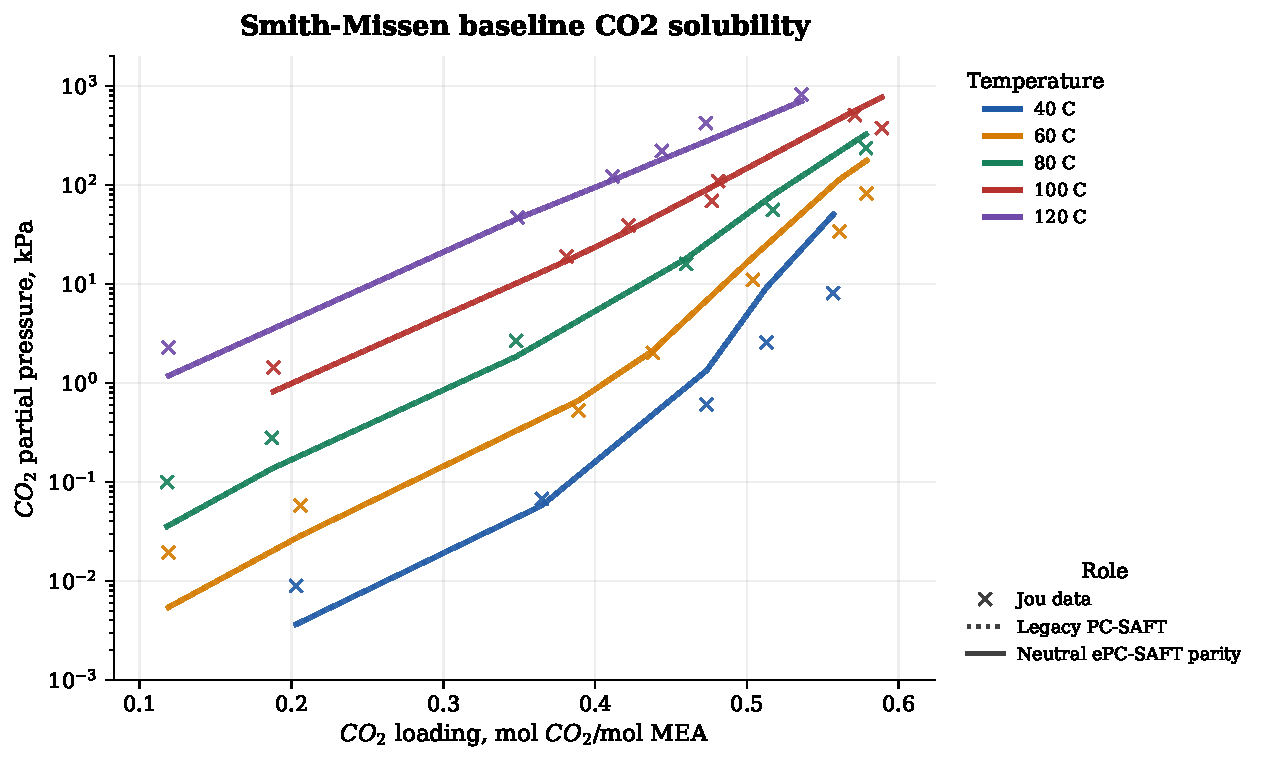
\includegraphics[width=0.84\linewidth,height=0.40\textheight,keepaspectratio]{figures/mea_ideal_pressure_vs_loading.pdf}
    \captionsetup{hypcap=false}
    \captionof{figure}{Ideal-equilibrium \COtwo-solubility pressure baseline for 30 wt\% \MEA.  Predicted pressure increases with loading at every temperature, with larger deviations at 40 and \SI{60}{\degreeCelsius} than at 80, 100, and \SI{120}{\degreeCelsius}.}
    \label{fig:ideal-pressure}
    \end{minipage}
\end{center}

\begin{center}
    \begin{minipage}{\linewidth}
    \centering
    \begin{minipage}{0.47\linewidth}
        \centering
        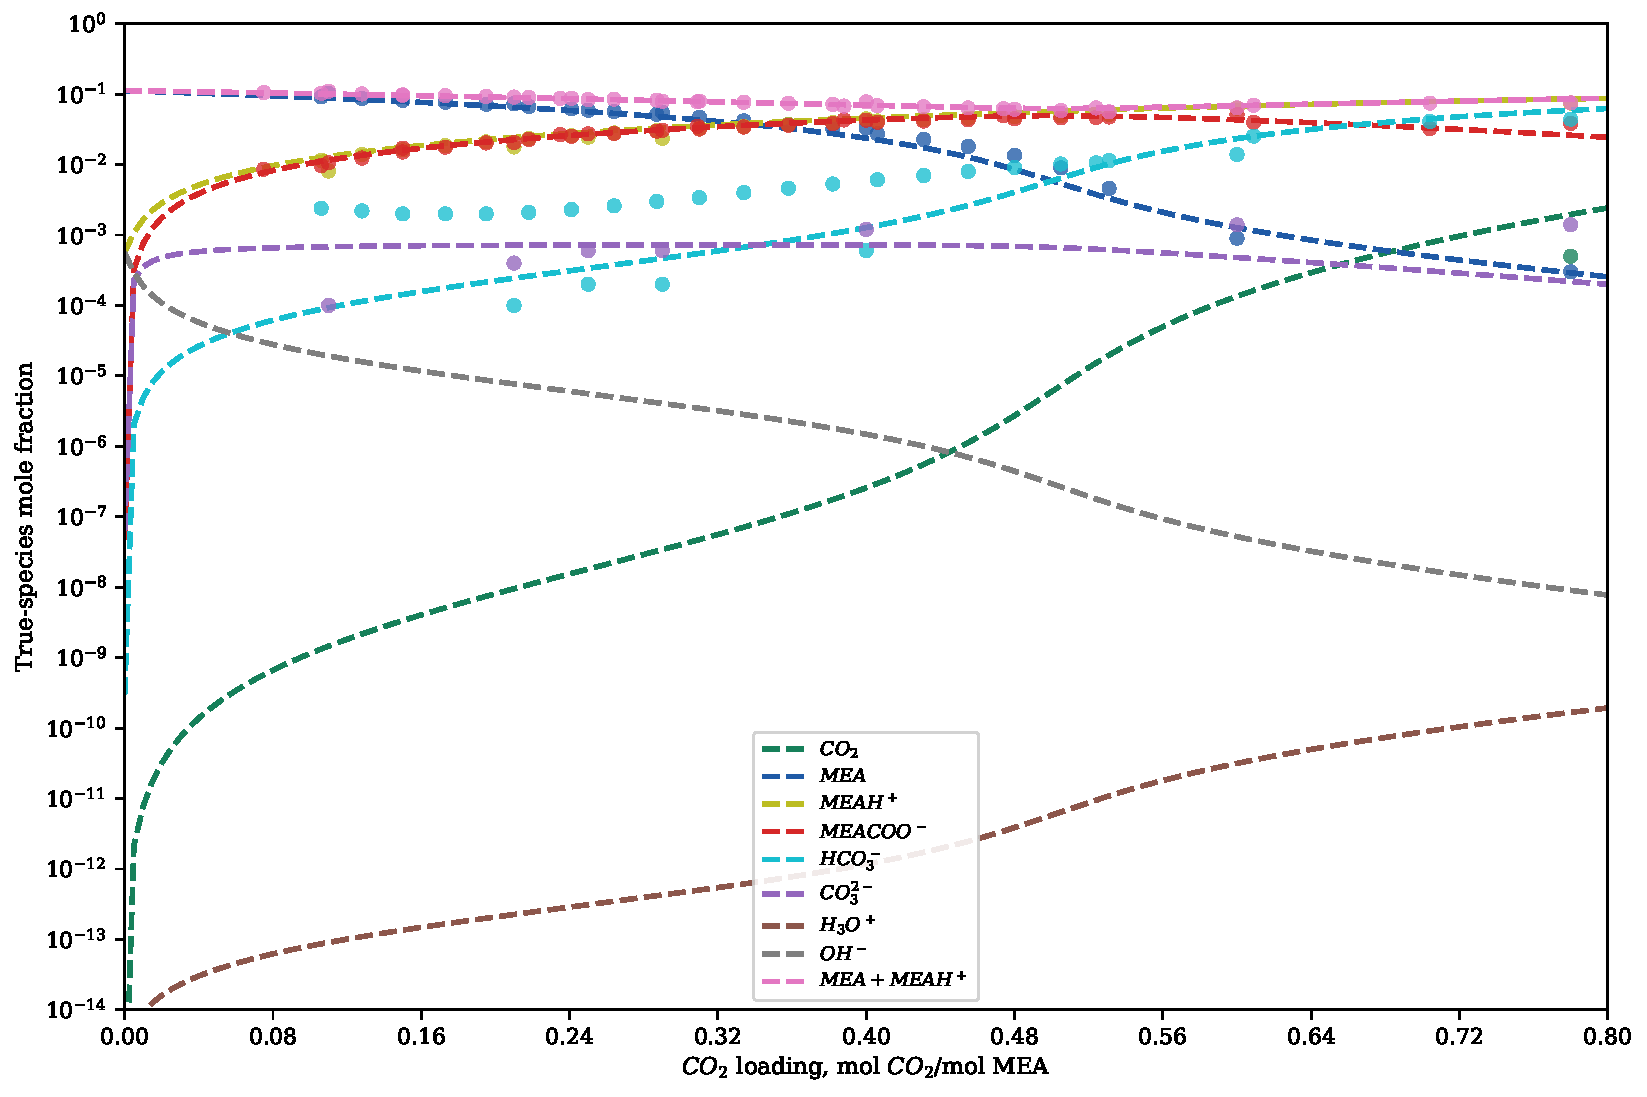
\includegraphics[width=\linewidth,height=0.30\textheight,keepaspectratio]{figures/mea_ideal_speciation_20C.pdf}
        \par\smallskip
        \small (a) \SI{20}{\degreeCelsius}
    \end{minipage}
    \hfill
    \begin{minipage}{0.47\linewidth}
        \centering
        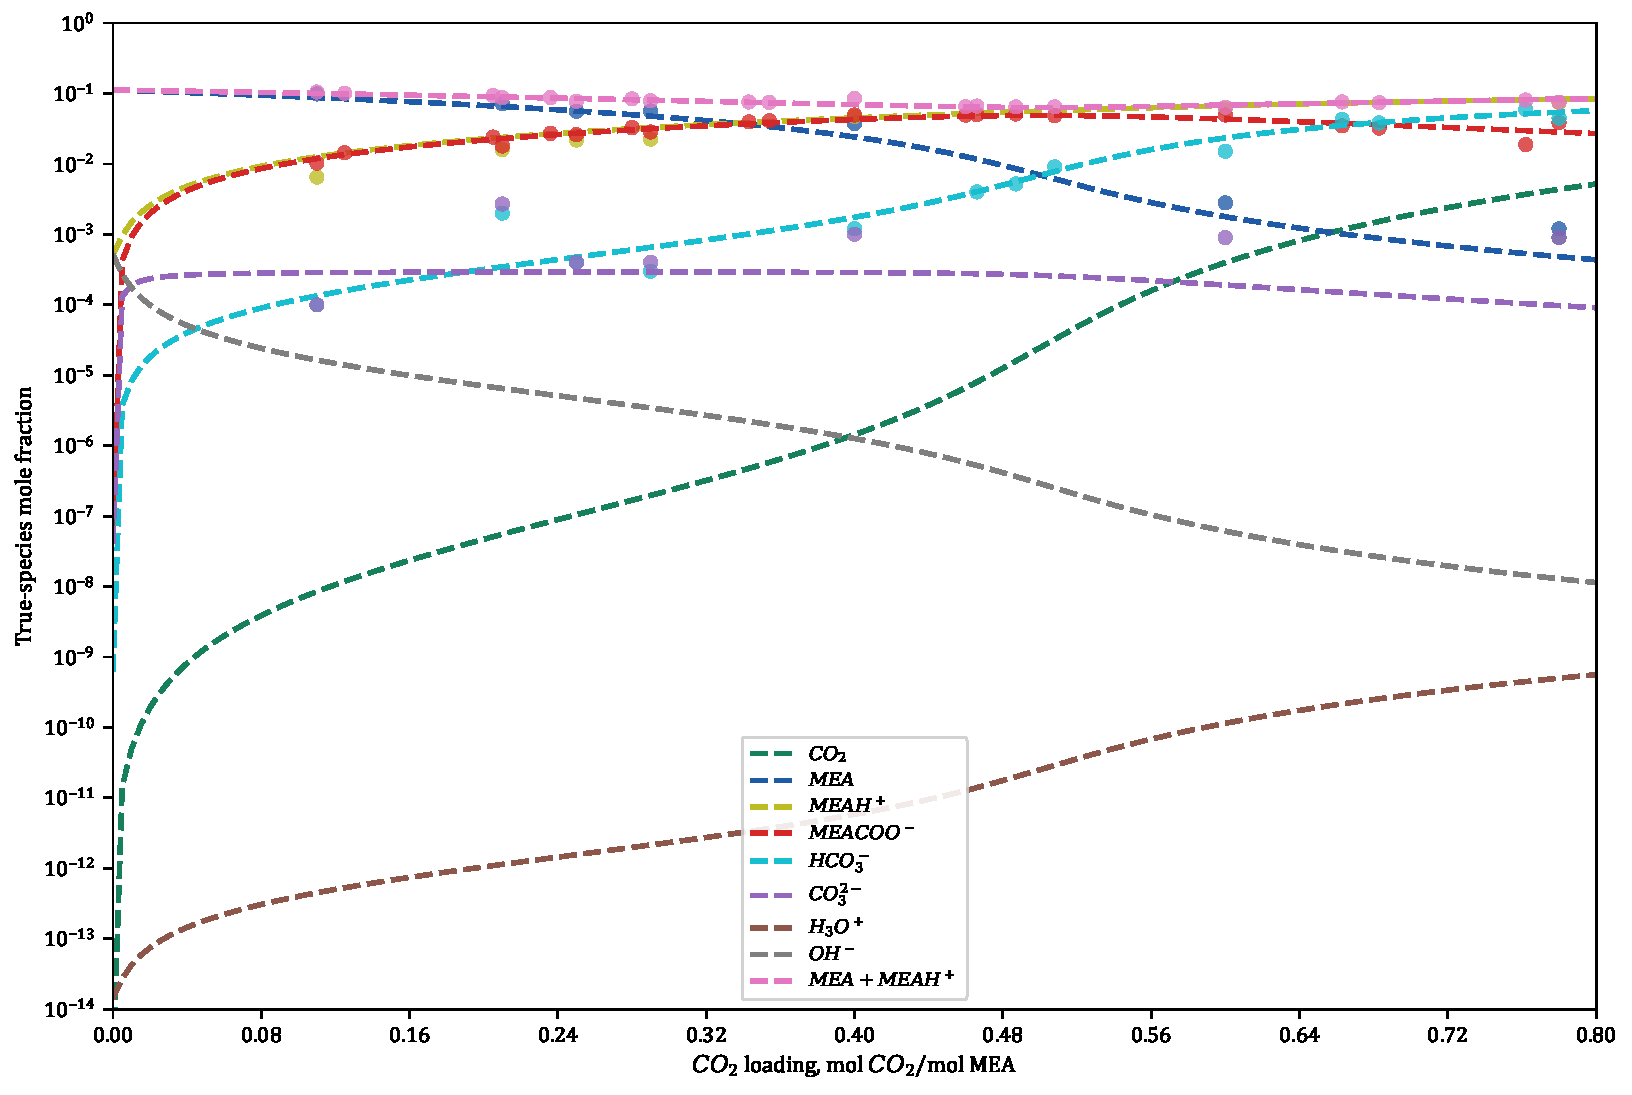
\includegraphics[width=\linewidth,height=0.30\textheight,keepaspectratio]{figures/mea_ideal_speciation_40C.pdf}
        \par\smallskip
        \small (b) \SI{40}{\degreeCelsius}
    \end{minipage}
    \captionsetup{hypcap=false}
    \captionof{figure}{Ideal-equilibrium true-species baseline for 30 wt\% \MEA.  Smooth curves show the five-reaction, nine-species equilibrium calculation; markers show literature values after declared composition-basis conversion.  Positive measured amine and bicarbonate values enter the residual comparison, while other species document the solved equilibrium state.}
    \label{fig:ideal-speciation}
    \end{minipage}
\end{center}

\subsection{Activity-based CO2 solubility model}
The activity calculation uses the nine-species basis and parameter hierarchy in \cref{sec:data-methods}.  As loading changes, it updates ionic composition, bulk permittivity, and modified-Born solvation within the activity coefficients.  The resulting liquid composition enters the \COtwo fugacity calculation, so one fixed thermodynamic state determines both pressure and speciation.

\subsection{Chemical speciation}
For the 66 NMR states excluded from parameter estimation, median absolute \(\log_{10}(\mathrm{model}/\mathrm{data})\) residuals for positive measurements are 0.065 for \MEA, 0.033 for \MEAH, 0.041 for \MEACOO, 0.452 for \HCOthree, 0.536 for \COthree, and 0.067 for \ce{MEA + MEAH+}.  At the 15 evaluation states where the source reports zero \HCOthree, the largest modeled mole fraction is 0.00147.  These values are upper-bound checks because the sources give no detection limits.

We excluded digitized Wong Raman values from the residual metrics because overlap-sensitive peak extraction and the composition-conversion denominator remain unresolved.  For the smooth activity curves, 642 of 644 requested states met the numerical acceptance criteria; the figures show those 642 states.

\begin{center}
    \begin{minipage}{\linewidth}
    \centering
    \begin{minipage}{0.47\linewidth}
        \centering
        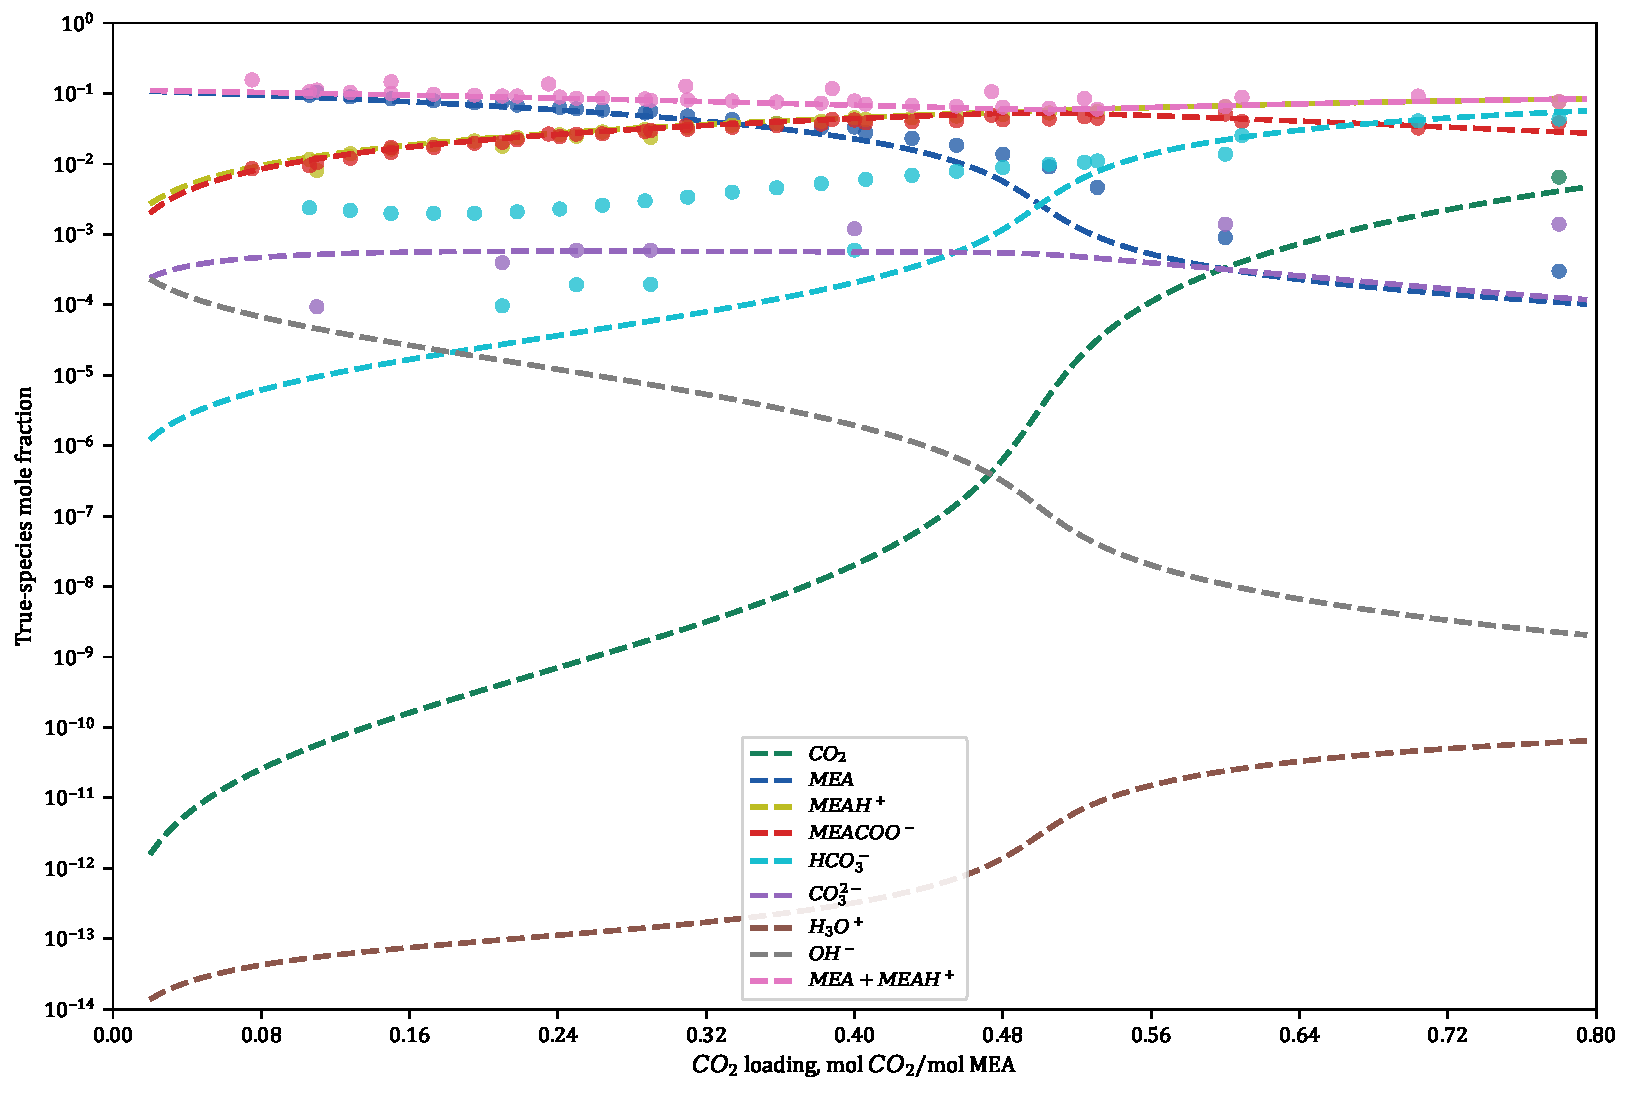
\includegraphics[width=\linewidth,height=0.27\textheight,keepaspectratio]{figures/mea_activity_speciation_20C.pdf}
        \par\smallskip
        \small (a) \SI{20}{\degreeCelsius}
    \end{minipage}
    \hfill
    \begin{minipage}{0.47\linewidth}
        \centering
        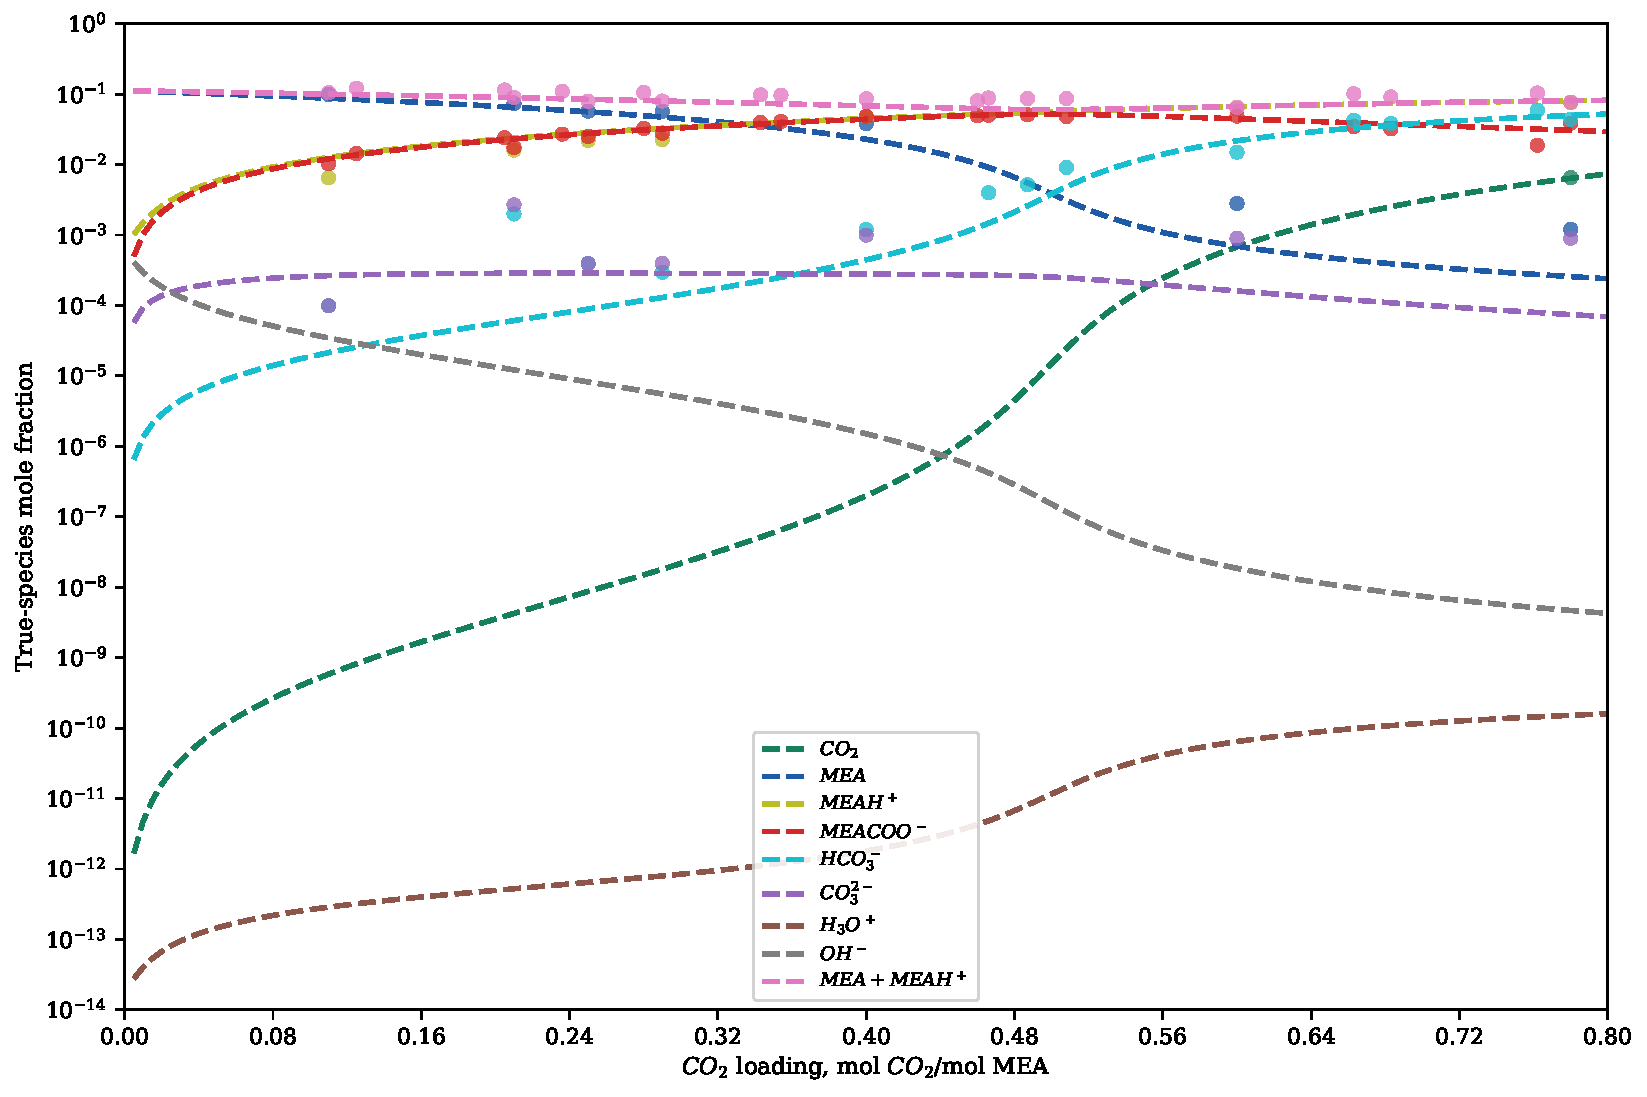
\includegraphics[width=\linewidth,height=0.27\textheight,keepaspectratio]{figures/mea_activity_speciation_40C.pdf}
        \par\smallskip
        \small (b) \SI{40}{\degreeCelsius}
    \end{minipage}
    \par\medskip
    \begin{minipage}{0.47\linewidth}
        \centering
        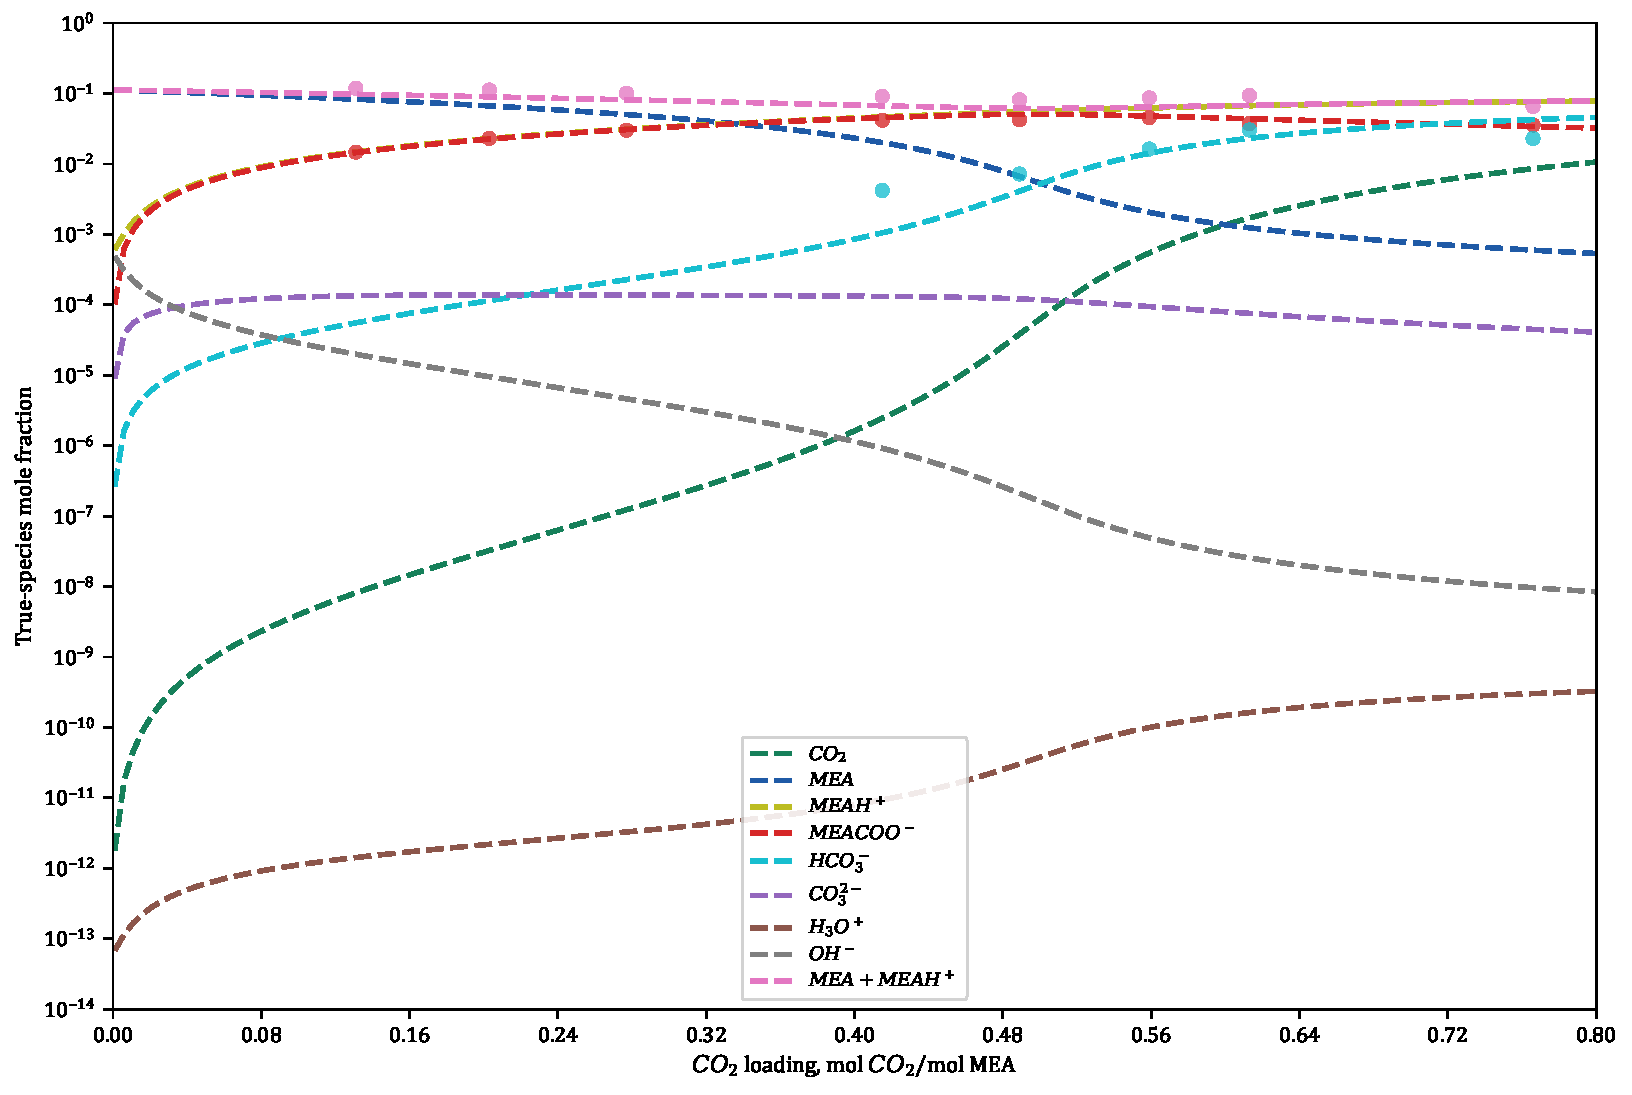
\includegraphics[width=\linewidth,height=0.27\textheight,keepaspectratio]{figures/mea_activity_speciation_60C.pdf}
        \par\smallskip
        \small (c) \SI{60}{\degreeCelsius}
    \end{minipage}
    \hfill
    \begin{minipage}{0.47\linewidth}
        \centering
        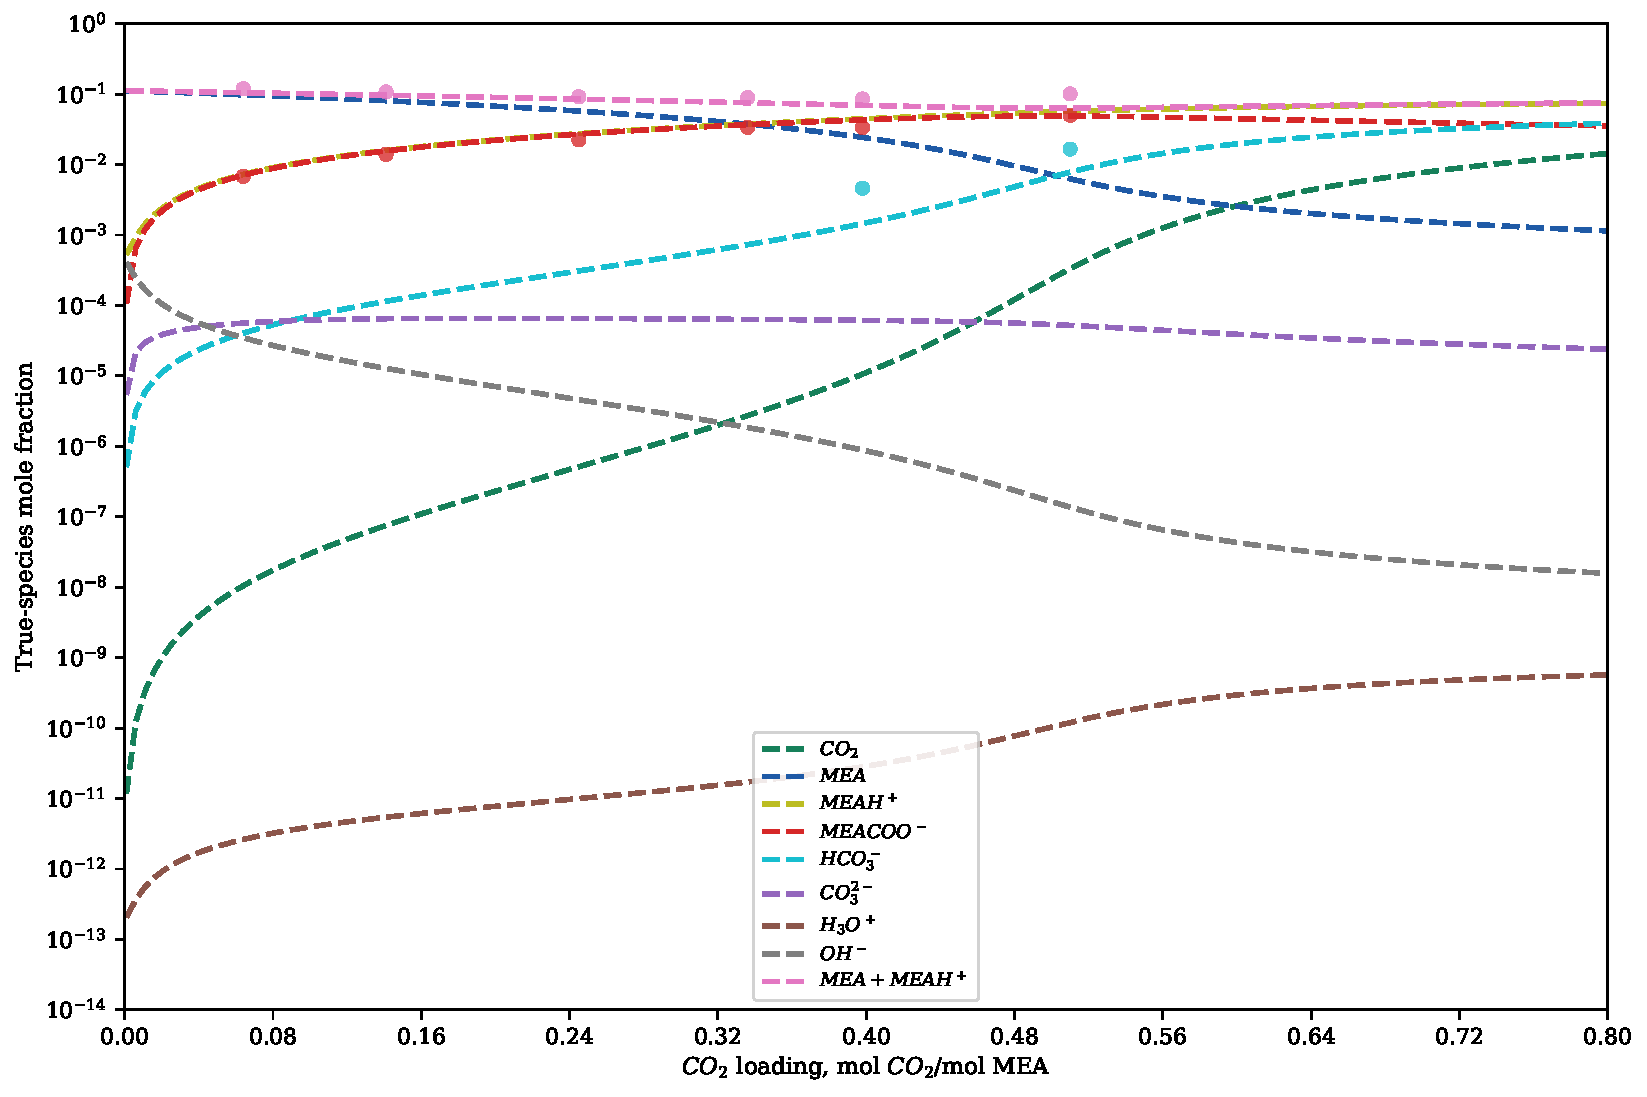
\includegraphics[width=\linewidth,height=0.27\textheight,keepaspectratio]{figures/mea_activity_speciation_80C.pdf}
        \par\smallskip
        \small (d) \SI{80}{\degreeCelsius}
    \end{minipage}
    \captionsetup{hypcap=false}
    \captionof{figure}{Activity-coupled ePC-SAFT speciation comparison for 30 wt\% \MEA.  Curves show the 642 accepted activity-coupled states, and markers show positive measured species or aggregate values.  Source-reported zero \HCOthree values enter upper-bound checks; balance-derived values are excluded from independent residuals.}
    \label{fig:activity-speciation}
    \end{minipage}
\end{center}

\subsection{CO2 solubility pressure response}
The controlled pressure comparison uses the same 31 Jou et al.\ measurements for both models.  The ideal baseline gives median absolute, signed median, and RMSE \(\log_{10}(P_{\mathrm{model}}/P_{\mathrm{data}})\) residuals of 0.160, \(-0.024\), and 0.297, respectively; the activity model gives 0.495, 0.226, and 0.565.  The activity model improves 4 paired records and worsens 27.  The ePC-SAFT parameterization therefore reduces pressure accuracy on this subset.

\begin{center}
    \begin{minipage}{\linewidth}
    \centering
    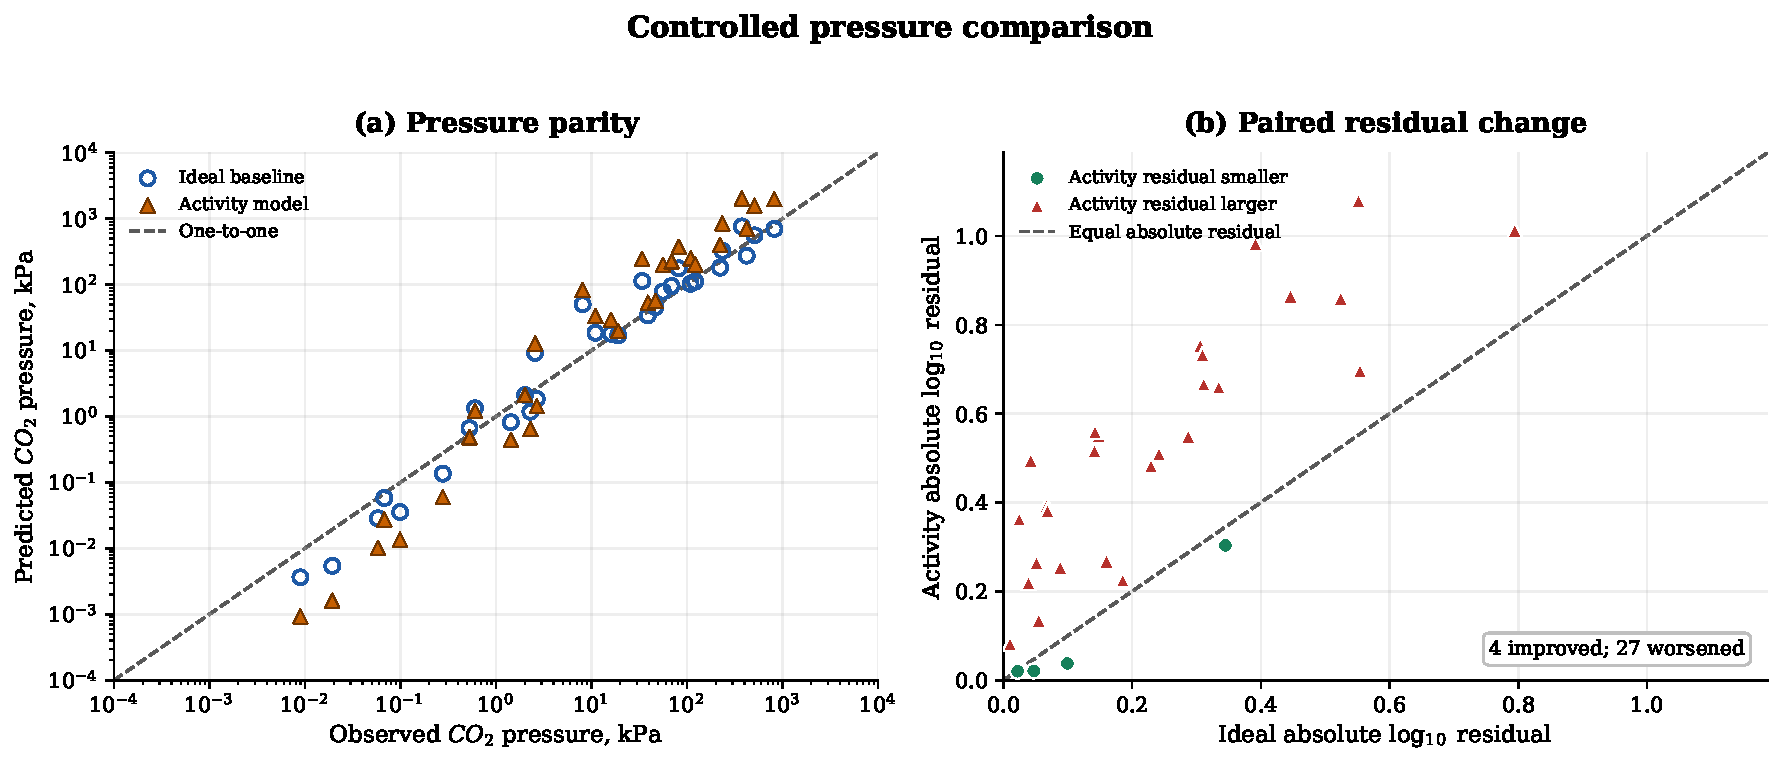
\includegraphics[width=0.96\linewidth,height=0.42\textheight,keepaspectratio]{figures/mea_controlled_pressure_comparison.pdf}
    \captionsetup{hypcap=false}
    \captionof{figure}{Controlled pressure evaluation using the same 31 Jou et al.\ measurements.  Panel (a) compares observed pressure with the ideal Smith--Missen baseline and activity-based ePC-SAFT calculation.  Panel (b) compares their absolute \(\log_{10}(P_{\mathrm{model}}/P_{\mathrm{data}})\) residuals; points below the one-to-one line favor the activity calculation.  The activity treatment reduces the absolute residual for 4 records and increases it for 27 records.}
    \label{fig:controlled-pressure-comparison}
    \end{minipage}
\end{center}

Across all 161 VLE records from six sources, the activity calculation gives median absolute, signed median, and RMSE pressure residuals of 0.493, \(-0.288\), and 0.645, respectively.  Because the ideal baseline was evaluated only on the 31-record Jou et al.\ subset, its metrics cannot be compared with this full-set summary.  The assembled pressure records contain no uncertainty values, so we report unweighted metrics.  Full-set pressure errors are largest between 40 and \SI{80}{\degreeCelsius} and decrease at \SI{120}{\degreeCelsius}.  The pressure residuals test gas--liquid equilibrium, while the NMR residuals test the liquid composition supporting that pressure.

\begin{center}
    \begin{minipage}{\linewidth}
    \centering
    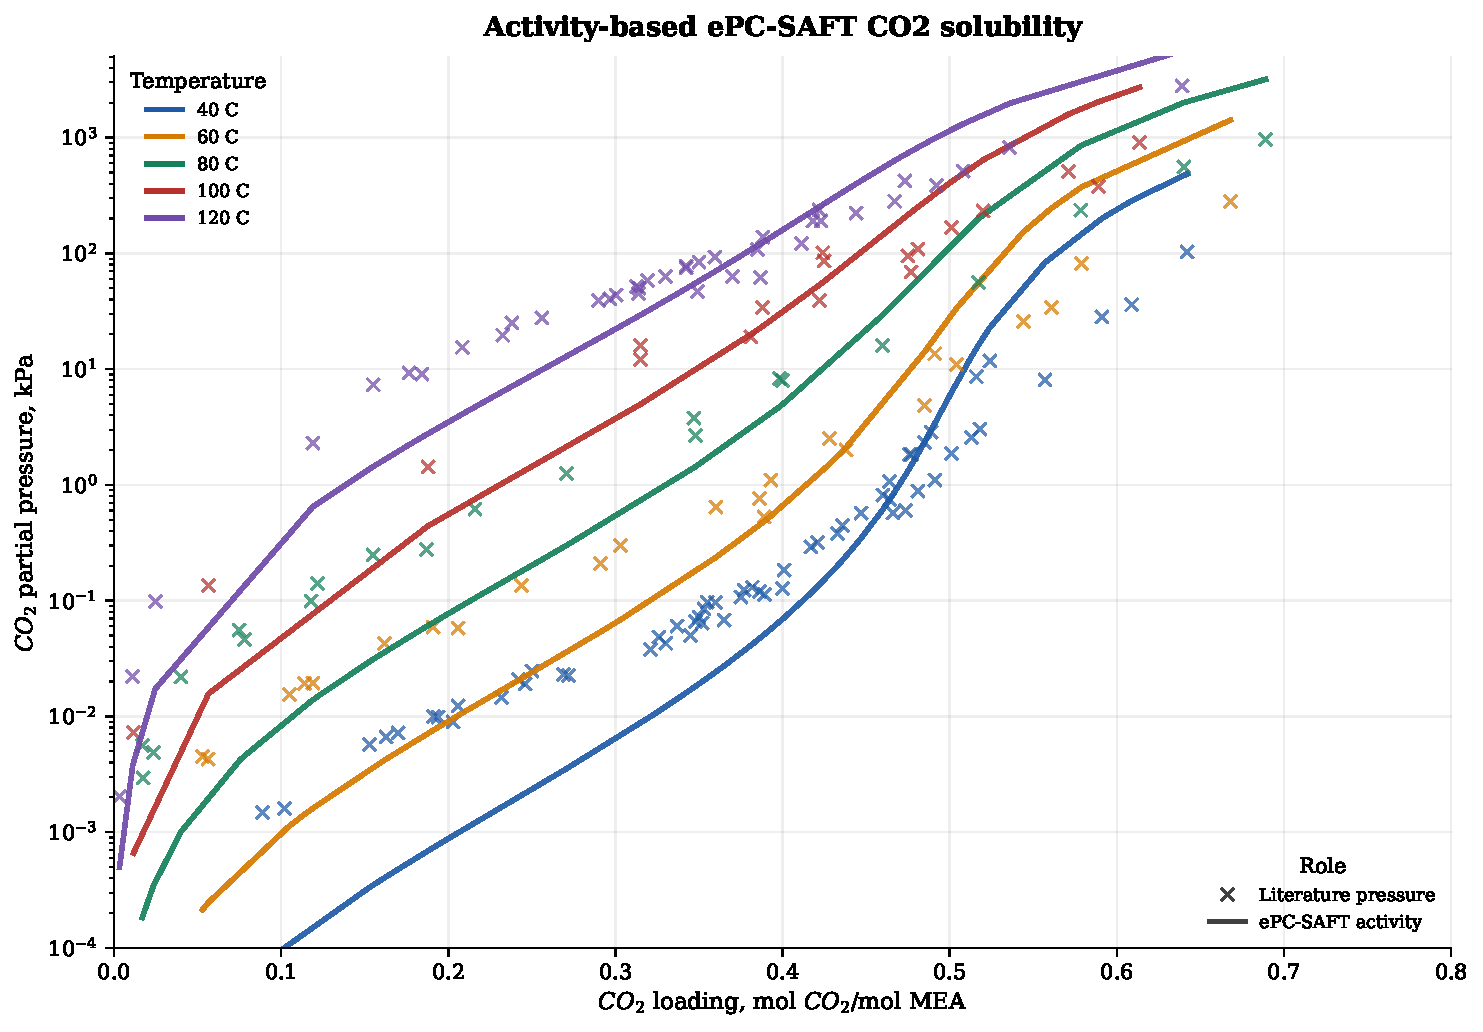
\includegraphics[width=0.84\linewidth,height=0.40\textheight,keepaspectratio]{figures/mea_activity_pressure_vs_loading.pdf}
    \captionsetup{hypcap=false}
    \captionof{figure}{Activity-coupled ePC-SAFT \COtwo-solubility pressure evaluation for 30 wt\% \MEA.  Connected curves show converged ePC-SAFT pressure rows at the assembled VLE loadings, and markers show the corresponding literature pressure records.}
    \label{fig:activity-pressure}
    \end{minipage}
\end{center}

\subsection{Sensitivity and identifiability}
The carbonate-family parameters are less identifiable than the amine-family parameters.  The NMR data include 53 positive \HCOthree and 16 positive \COthree observations, compared with 74 direct \MEACOO observations and 74 direct \ce{MEA + MEAH+} aggregate observations.  The reported calculation uses \(d_{\HCOthree}^{\mathrm{Born}}=3.0\) and \(d_{\COthree}^{\mathrm{Born}}=3.0\).  A carbonate-only sensitivity scan lowers the carbonate residual near \(d_{\HCOthree}^{\mathrm{Born}}=6.80\) and \(d_{\COthree}^{\mathrm{Born}}=3.00\).  We retain the 3.0/3.0 pair because the alternative is identified only by the carbonate observations used in the scan and lacks an independent pressure/speciation test.  \HthreeO and \Hydroxide are determined mainly by electroneutrality and water autoionization; the available NMR data provide no independent observations for either ion.

\begin{center}
    \begin{minipage}{\linewidth}
    \centering
    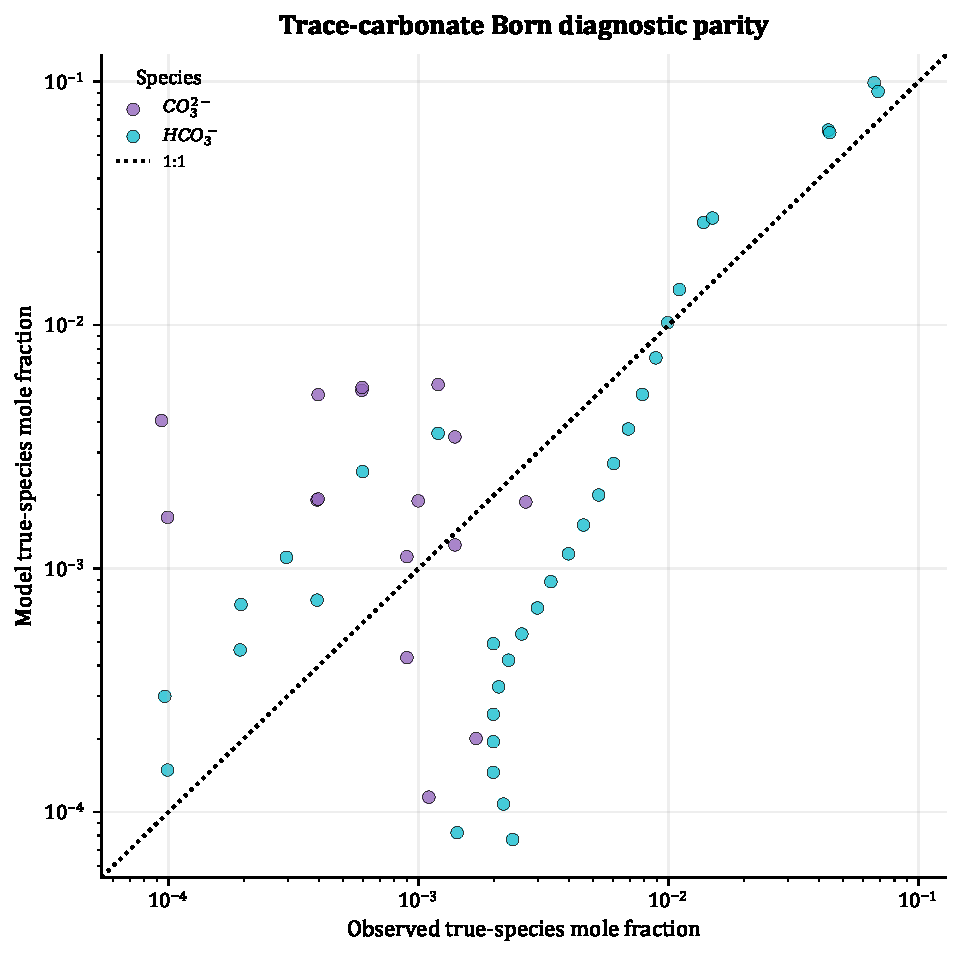
\includegraphics[width=0.64\linewidth,height=0.36\textheight,keepaspectratio]{figures/trace_carbonate_born_parity.pdf}
    \captionsetup{hypcap=false}
    \captionof{figure}{Carbonate-only Born-diameter sensitivity for \HCOthree and \COthree.  The reported calculation uses the 3.0/3.0 pair; the sensitivity scan shows that bicarbonate residuals vary strongly with the bicarbonate Born diameter.}
    \label{fig:trace-carbonate-born-regression}
    \end{minipage}
\end{center}

\subsection{Comparison with literature models}
\Cref{tab:literature-model-comparison} distinguishes apparent-chemistry PC-SAFT treatments, explicit-ion ePC-SAFT amine models, and advanced-Born electrolyte models for gas solubility.  The present calculation applies explicit-ion activity coupling and SSM+DS modified-Born solvation to carbamate-forming \MEA.  Following prior ePC-SAFT amine-solubility studies, the parameter estimation uses liquid-composition data while the VLE data test the predicted pressure~\cite{Uyan2015,Wangler2018}.

\subsection{Model limitations}
The seven fitted parameters reduce the squared NMR residual objective by 2.8\%, and the evaluation residuals remain much larger for bicarbonate and carbonate than for the amine family.  A local finite-difference screen is most sensitive to \(k_{\MEA,\HtwoO}\), \(k_{\COtwo,\MEA}\), and \(d_{\COthree}^{\mathrm{Born}}\); \(d_{\HthreeO}^{\mathrm{Born}}\) has little effect on the reported metrics.  The pressure comparison also shows that agreement with liquid speciation does not guarantee an accurate \COtwo pressure response.

\section{Conclusions}\label{sec:conclusion}
We developed a nine-species SSM+DS modified-Born ePC-SAFT model for 30 wt\% aqueous \MEA.  Seven \MEAH/\MEACOO parameters were fitted to 22 composition residuals from eight NMR states.  The calculation converged at all 161 pressure records and 74 NMR states.

On the 66 NMR states excluded from parameter estimation, median absolute \(\log_{10}(\mathrm{model}/\mathrm{data})\) residuals were 0.065 for \MEA, 0.033 for \MEAH, 0.041 for \MEACOO, 0.452 for \HCOthree, 0.536 for \COthree, and 0.067 for the \ce{MEA + MEAH+} aggregate.  The model therefore describes the measured amine-family composition more closely than the carbonate family.

The pressure results remain less accurate than the ideal-activity baseline.  On the same 31 Jou et al.\ measurements, the median absolute \(\log_{10}(P_{\mathrm{model}}/P_{\mathrm{data}})\) residual was 0.160 for the ideal baseline and 0.495 for ePC-SAFT.  Across all 161 pressure records, the ePC-SAFT median absolute residual was 0.493.  The combined pressure and speciation comparison shows that the present ionic parameterization captures the dominant amine species more accurately than carbonate speciation or the equilibrium pressure.

\section*{Data and Code Availability}
The processed evaluation tables, including the source-resolved pressure/speciation residual summary, retained parameter tables, plotting CSV files, and source identifiers used in this manuscript are maintained with the public source repository at \url{https://github.com/tannerpolley/MEA-Thermodynamics}.  The exact evaluation environment is locked to \texttt{epcsaft} 1.5.2 at Git commit \texttt{9f51afd0f9c11a6497ddca05c8b2dd0ea0ffa785}.  An immutable repository release and archival DOI have not yet been published; these identifiers and the repository license remain corresponding-author decisions to be completed before submission.

\section*{Funding}
This research received no specific grant from funding agencies in the public, commercial, or not-for-profit sectors.

\section*{Declaration of Competing Interest}
The author declares no known competing financial interests or personal relationships that could have appeared to influence the work reported in this paper.

\section*{CRediT Author Statement}
Tanner W. Polley: Conceptualization, methodology, software, validation, formal analysis, investigation, data curation, writing--original draft, writing--review and editing, and visualization.

\section*{Declaration of Generative AI and AI-Assisted Technologies}
During preparation of this manuscript, AI-assisted tools were used for editorial review, language polishing, and computational consistency checks.  The author reviewed and edited the content and takes responsibility for the final manuscript.


\clearpage
\bibliographystyle{styles/model1-num-names}
\bibliography{manuscript_references,project_sources,official_sources}

\clearpage
\vspace*{\fill}
\phantomsection
\noindent\begin{minipage}{\linewidth}
    \centering
    \captionsetup{hypcap=false,justification=raggedright,singlelinecheck=false,labelfont=bf,labelsep=newline}
    \captionof{table}{Primary symbols used in this manuscript.}
    \label{tab:nomenclature}
    \begin{tabularx}{\linewidth}{lX}
        \toprule
        Symbol & Definition \\
        \midrule
        \(L\) & \COtwo loading on \MEA (mol \COtwo per mol apparent \MEA) \\
        \(T\) & Temperature \\
        \(P\) & Total pressure \\
        \(P_{\mathrm{CO_2}}\) & \COtwo equilibrium partial pressure \\
        \(y_i, x_i\) & Gas- and liquid-phase molar composition of species \(i\) \\
        \(z_i^{\mathrm{app}}\) & Apparent liquid-state mole fraction of apparent species \(i\) \\
        \(x_i^{\mathrm{true}}\) & True-species liquid mole fraction of species \(i\) after speciation solve \\
        \(\gamma_i\) & Species activity coefficient from ePC-SAFT \\
        \(\phi_i\) & Fugacity coefficient from ePC-SAFT \\
        \(k_{ij}\) & Binary dispersion interaction parameter between species \(i\) and \(j\) \\
        \(\kappa\) & Inverse Debye length in the electrolyte contribution \\
        \(\kappa^{A_iB_j}_{ij}\) & Association-volume parameter for sites \(A_i\) and \(B_j\) \\
        \(\sigma_i,\epsilon_i\) & PC-SAFT segment diameter and energy parameters for species \(i\) \\
        \(\lambda^{\mathrm{Born}}\) & Species-specific Born correction parameter \\
        \(\mathbf{R}\) & Charge/atom-balance constraints in speciation solves \\
        \text{RMSE} & Root-mean-square error (defined on the transformed residual scale indicated in text) \\
        \bottomrule
    \end{tabularx}
\end{minipage}\par


\end{document}

